\documentclass{beamer}
\usepackage{bbding}
\usepackage{pifont}
\usepackage{wasysym}
\usepackage{amssymb}
\usepackage{animate}
\usepackage{float}
\usepackage{bm}
\usepackage{mathtools}
\usepackage{extarrows}
\usepackage{amssymb}% http://ctan.org/pkg/amssymb
\usepackage{pifont}% http://ctan.org/pkg/pifont
\newcommand{\cmark}{\ding{51}}%
\newcommand{\xmark}{\ding{55}}%
\usepackage{booktabs}

\newcommand{\ChoL}{\mathsf{L}}
\newcommand{\ii}{\mathrm{i}}
\newcommand{\bxi}{\bm{\xi}}
\newcommand{\bmu}{\bm{\mu}}
\newcommand{\bb}{\mathbf{b}}
\newcommand{\bA}{\mathbf{A}}
\newcommand{\bJ}{\mathbf{J}}
\newcommand{\bB}{\mathbf{B}}
\newcommand{\bM}{\mathbf{M}}

\newcommand{\by}{\mathbf{y}}
\newcommand{\bw}{\mathbf{w}}

\newcommand{\bY}{\mathbf{Y}}
\newcommand{\bs}{\mathbf{s}}
\newcommand{\sign}{\mathrm{sign}}
\newcommand{\bc}{\mathbf{c}}
\newcommand{\bzero}{\mathbf{0}}
\renewcommand{\bf}{\mathbf{f}}
\newcommand{\bu}{\mathbf{u}}
\newcommand{\bv}[0]{\mathbf{v}}

\mode<presentation> {

% The Beamer class comes with a number of default slide themes
% which change the colors and layouts of slides. Below this is a list
% of all the themes, uncomment each in turn to see what they look like.

%\usetheme{default}
%\usetheme{AnnArbor}
%\usetheme{Antibes}
%\usetheme{Bergen}
%\usetheme{Berkeley}
%\usetheme{Berlin}
%\usetheme{Boadilla}
%\usetheme{CambridgeUS}
%\usetheme{Copenhagen}
%\usetheme{Darmstadt}
%\usetheme{Dresden}
%\usetheme{Frankfurt}
%\usetheme{Goettingen}
%\usetheme{Hannover}
%\usetheme{Ilmenau}
%\usetheme{JuanLesPins}
%\usetheme{Luebeck}
\usetheme{Madrid}
%\usetheme{Malmoe}
%\usetheme{Marburg}
%\usetheme{Montpellier}
%\usetheme{PaloAlto}
%\usetheme{Pittsburgh}
%\usetheme{Rochester}
%\usetheme{Singapore}
%\usetheme{Szeged}
%\usetheme{Warsaw}


% As well as themes, the Beamer class has a number of color themes
% for any slide theme. Uncomment each of these in turn to see how it
% changes the colors of your current slide theme.

%\usecolortheme{albatross}
\usecolortheme{beaver}
%\usecolortheme{beetle}
%\usecolortheme{crane}
%\usecolortheme{dolphin}
%\usecolortheme{dove}
%\usecolortheme{fly}
%\usecolortheme{lily}
%\usecolortheme{orchid}
%\usecolortheme{rose}
%\usecolortheme{seagull}
%\usecolortheme{seahorse}
%\usecolortheme{whale}
%\usecolortheme{wolverine}

%\setbeamertemplate{footline} % To remove the footer line in all slides uncomment this line
%\setbeamertemplate{footline}[page number] % To replace the footer line in all slides with a simple slide count uncomment this line

%\setbeamertemplate{navigation symbols}{} % To remove the navigation symbols from the bottom of all slides uncomment this line
}
\usepackage{booktabs}
\usepackage{makecell}
\usepackage{soul}
\newcommand{\red}[1]{\textcolor{red}{#1}}
%
%\usepackage{graphicx} % Allows including images
%\usepackage{booktabs} % Allows the use of \toprule, \midrule and \bottomrule in tables
%
%
%\usepackage{amsthm}
%
%\usepackage{todonotes}
%\usepackage{floatrow}
%
%\usepackage{pgfplots,algorithmic,algorithm}
\usepackage{algorithmicx}
\usepackage{algpseudocode}
%\usepackage[toc,page]{appendix}
%\usepackage{float}
%\usepackage{booktabs}
%\usepackage{bm}
%
%\theoremstyle{definition}
%
\newcommand{\RR}[0]{\mathbb{R}}
%
%\newcommand{x}{\mathbf{x}}
%\newcommand{\ii}{\mathrm{i}}
%\newcommand{xi}{\bm{\xi}}
%\newcommand{\bmu}{\bm{\mu}}
%\newcommand{\bb}{\mathbf{b}}
%\newcommand{\bA}{\mathbf{A}}
%\newcommand{\bJ}{\mathbf{J}}
%\newcommand{\bB}{\mathbf{B}}
%\newcommand{\bM}{\mathbf{M}}
%\newcommand{\bF}{\mathbf{F}}
%
%\newcommand{\by}{\mathbf{y}}
%\newcommand{\bw}{\mathbf{w}}
%\newcommand{\bn}{\mathbf{n}}
%
%\newcommand{x}{\mathbf{X}}
%\newcommand{\bY}{\mathbf{Y}}
%\newcommand{\bs}{\mathbf{s}}
%\newcommand{\sign}{\mathrm{sign}}
%\newcommand{\theta}[0]{\bm{\theta}}
%\newcommand{\bc}{\mathbf{c}}
%\newcommand{\bzero}{\mathbf{0}}
%\renewcommand{\bf}{\mathbf{f}}
%\newcommand{\bu}{\mathbf{u}}
%\newcommand{\bv}[0]{\mathbf{v}}

\AtBeginSection[]
{
   \begin{frame}
       \frametitle{Outline}
       \tableofcontents[currentsection]
   \end{frame}
}

%----------------------------------------------------------------------------------------
%    TITLE PAGE
%----------------------------------------------------------------------------------------
\usepackage{bm}
\newcommand*{\TakeFourierOrnament}[1]{{%
\fontencoding{U}\fontfamily{futs}\selectfont\char#1}}
\newcommand*{\danger}{\TakeFourierOrnament{66}}

\title[Inverse Problem]{Physics Based Machine Learning for Inverse Problems} % The short title appears at the bottom of every slide, the full title is only on the title page

\author[CME 216]{Kailai Xu and Eric Darve} % Your name
%\institute[] % Your institution as it will appear on the bottom of every slide, may be shorthand to save space
%{
%%ICME, Stanford University \\ % Your institution for the title page
%%\medskip
%%\textit{kailaix@stanford.edu}\quad \textit{darve@stanford.edu} % Your email address
%}
\date{}% Date, can be changed to a custom date
% Mathematics of PDEs


\begin{document}

%\usebackgroundtemplate{%
%\begin{picture}(0,250)
%\centering
%	{{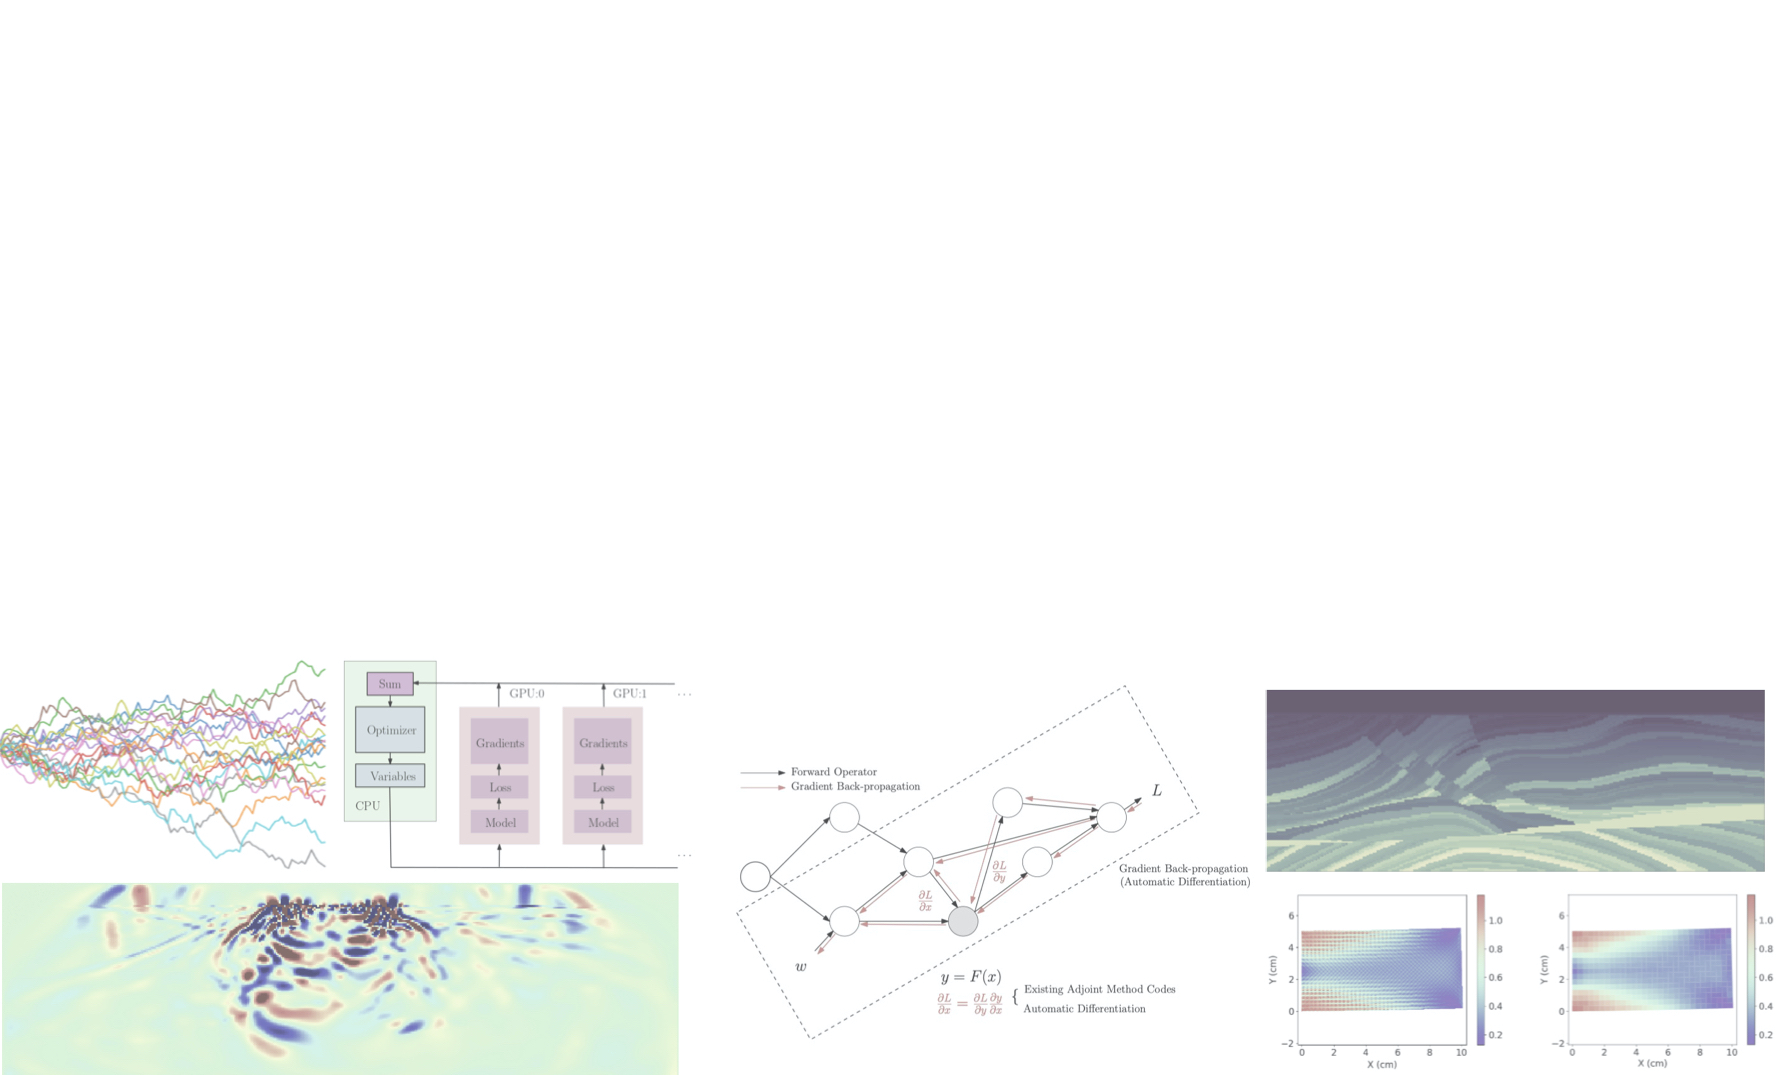
\includegraphics[width=1.0\paperwidth]{figures/background}}}
%\end{picture}
%  } 
%\usebackgroundtemplate{%
%  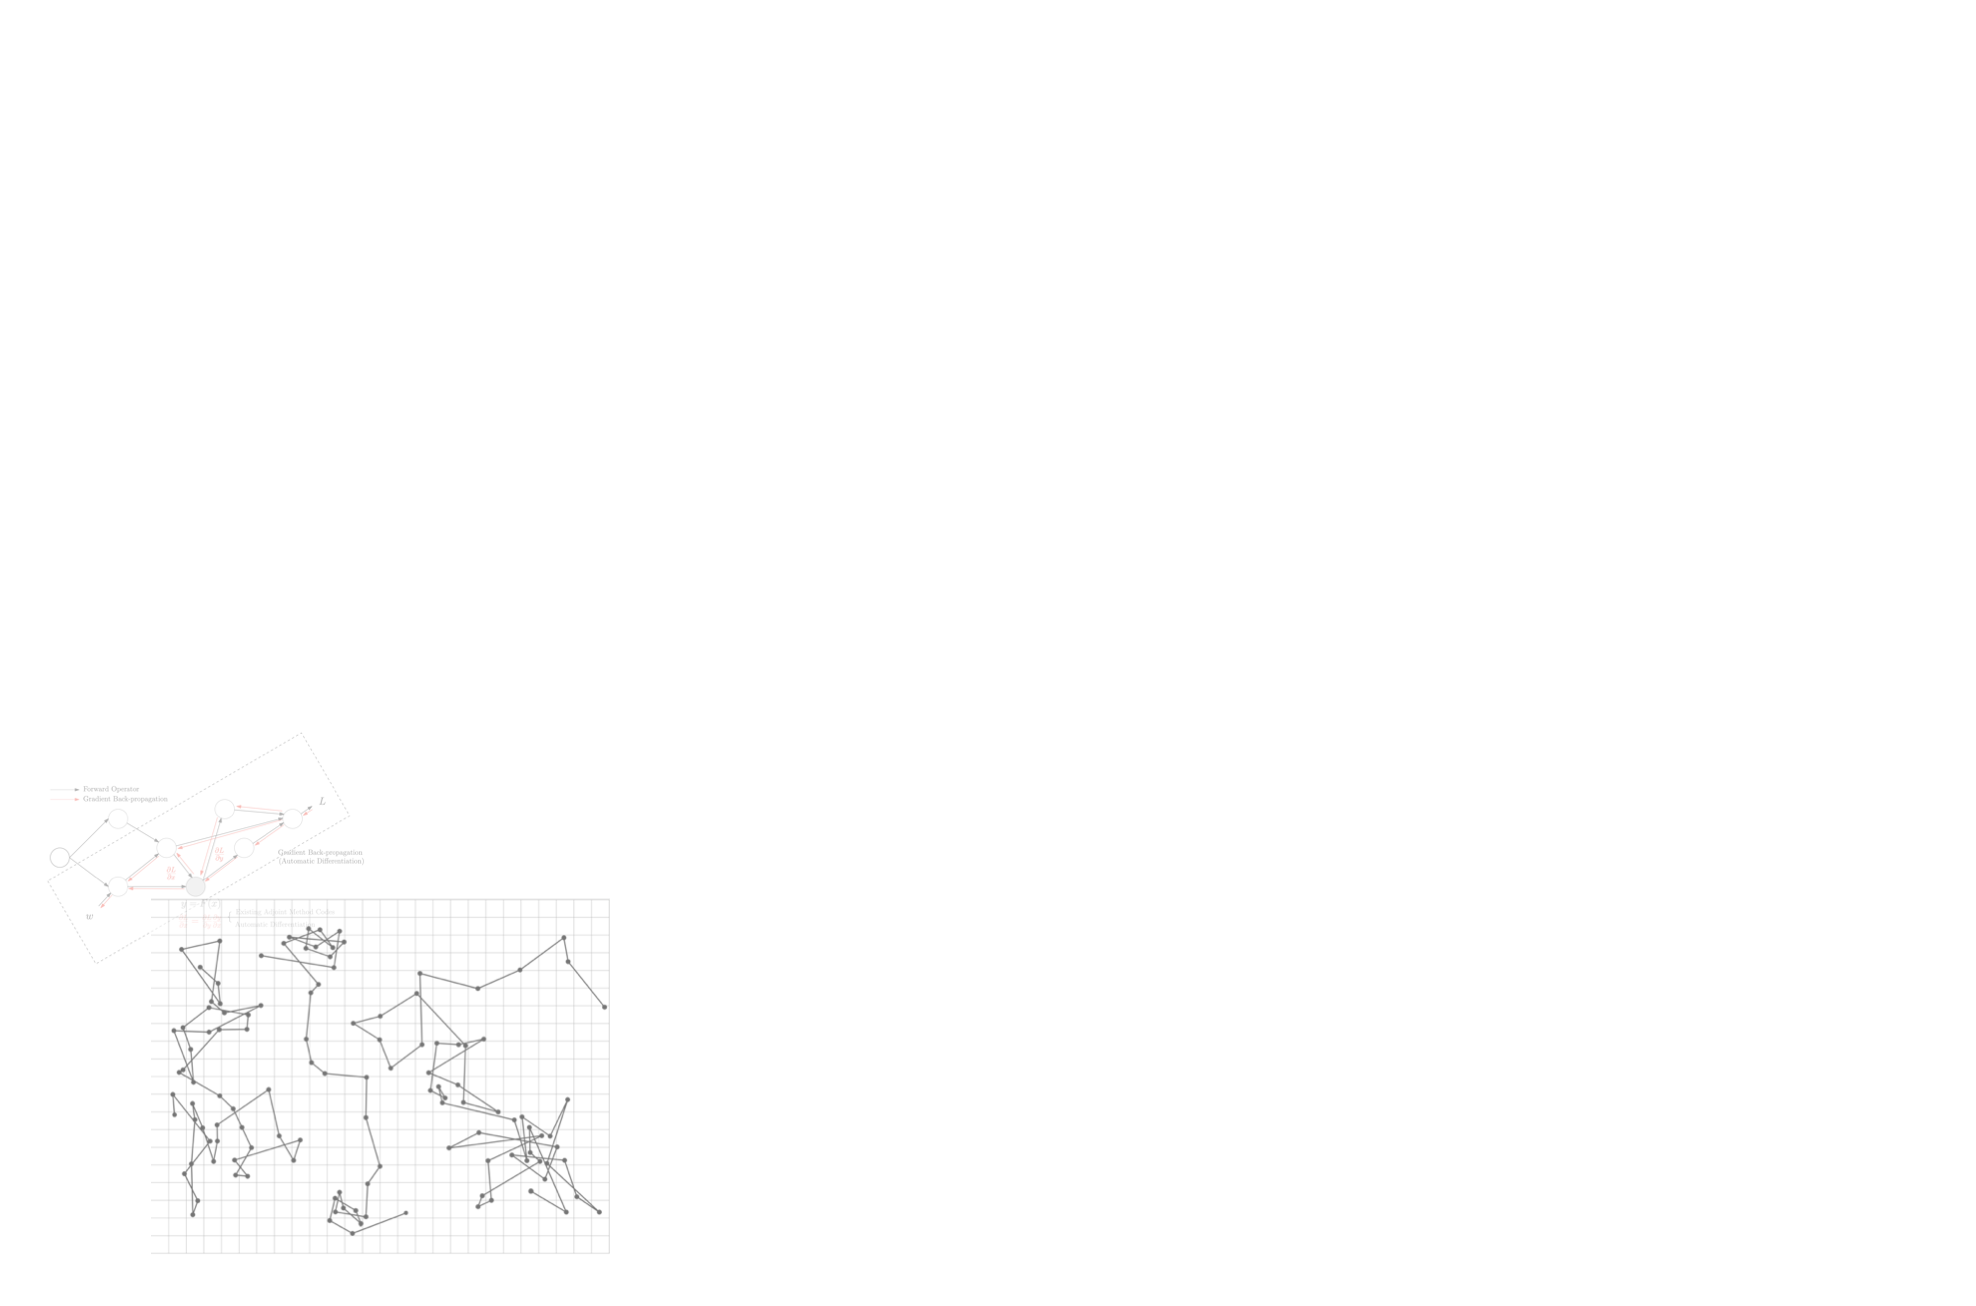
\includegraphics[width=\paperwidth,height=\paperheight]{figures/back}} 
\begin{frame}

\titlepage % Print the title page as the first slide

%dfa
\end{frame}
%\usebackgroundtemplate{}

\section{Inverse Problem}

\begin{frame}
	\frametitle{Recap: Inverse Problem in Heat Transfer}
	\begin{itemize}
\item Goal: calibrate $a$ and $b$ from $u_0(t) = u(0, t)$
$$\kappa(x) = a + bx$$
	\end{itemize}	
	\begin{figure}
		\centering
		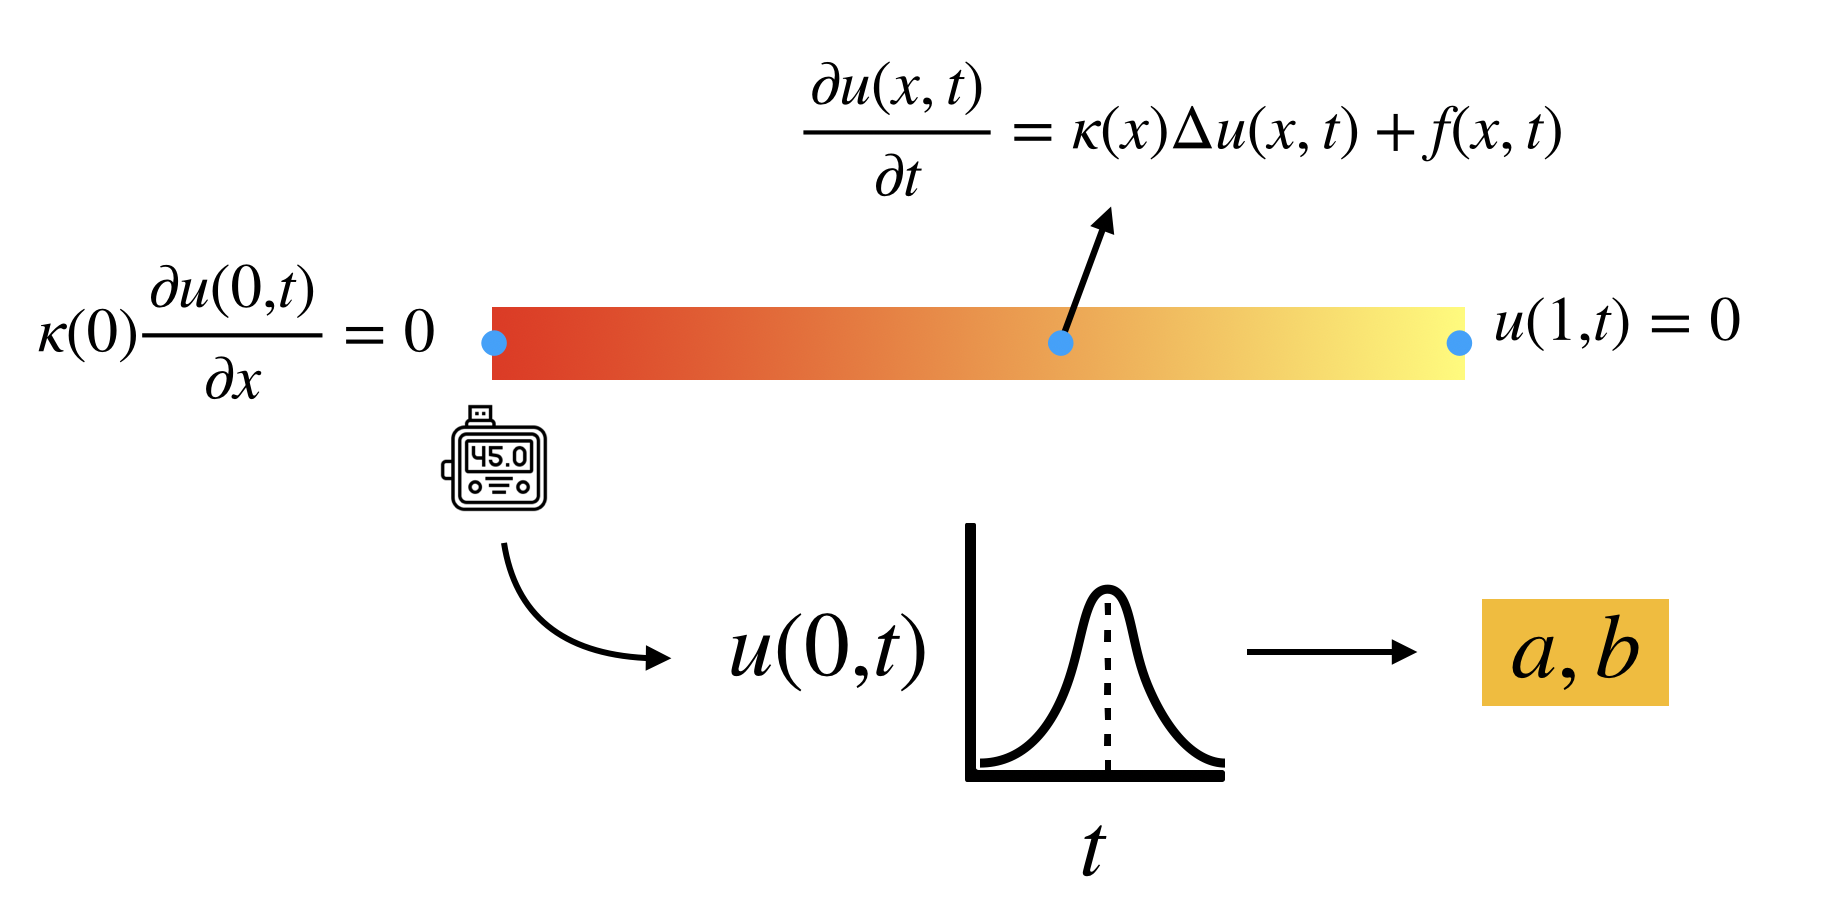
\includegraphics[width=1.0\textwidth]{figures/measure}
	\end{figure}

\end{frame}

\begin{frame}
	\frametitle{Mathematical Points of View}
	\begin{itemize}
		\item This problem is a standard inverse problem. We can formulate the problem as a PDE-constrained optimization problem
		$$\begin{aligned}
\min_{a, b}\ & \int_{0}^t ( u(0, t)- u_0(t))^2 dt\\
\mathrm{s.t.}\ & \frac{\partial u(x, t)}{\partial t} = \kappa(x)\Delta u(x, t) + f(x, t), \quad t\in (0,T), x\in (0,1) \\
& -\kappa(0)\frac{\partial u(0,t)}{\partial x} = 0, t>0\\
& u(1, t) = 0, t>0\\
& u(x, 0) = 0, x\in [0,1]\\
& \kappa(x) = a x + b
\end{aligned}$$

	\end{itemize}
\end{frame}





\begin{frame}
	\frametitle{Inverse Modeling}
	\begin{figure}
	\centering
  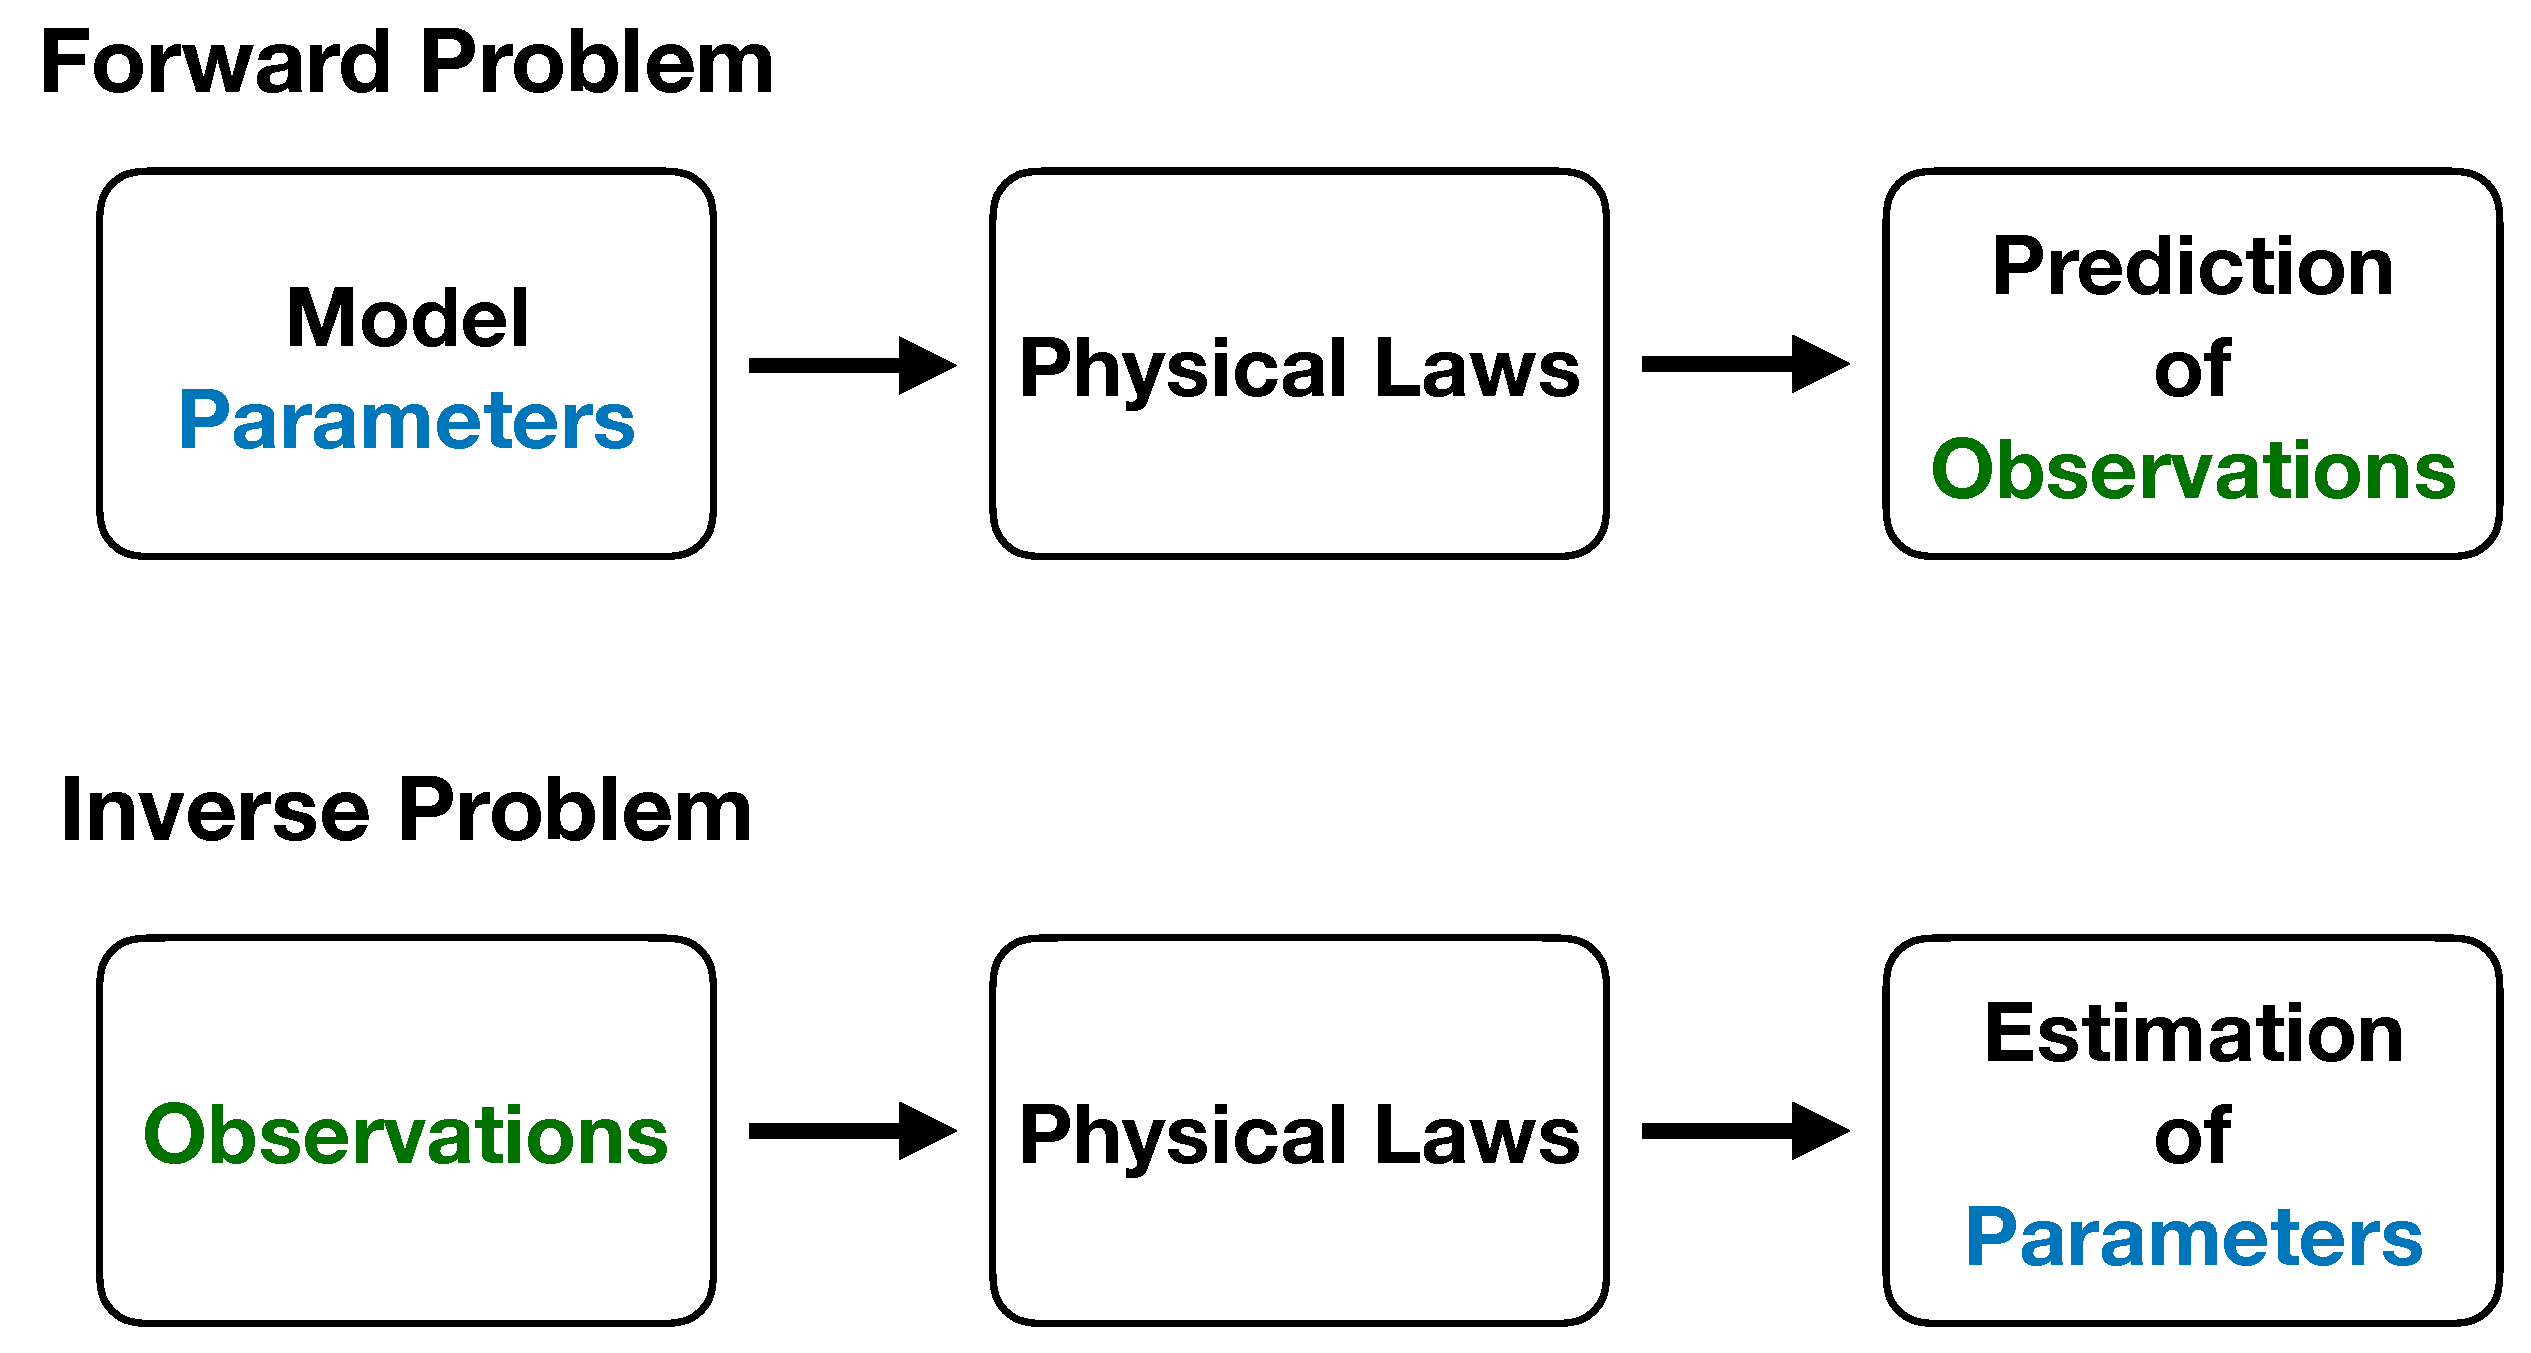
\includegraphics[width=1.0\textwidth]{figures/inverse3}
\end{figure}
\end{frame}

\begin{frame}
	\frametitle{Inverse Modeling}
	\begin{itemize}
		\item Many real life engineering problems can be formulated as inverse modeling problems: shape optimization for improving the performance of structures, optimal control of fluid dynamic systems, etc.
	\end{itemize}
	\begin{figure}[hbt]
	\centering
  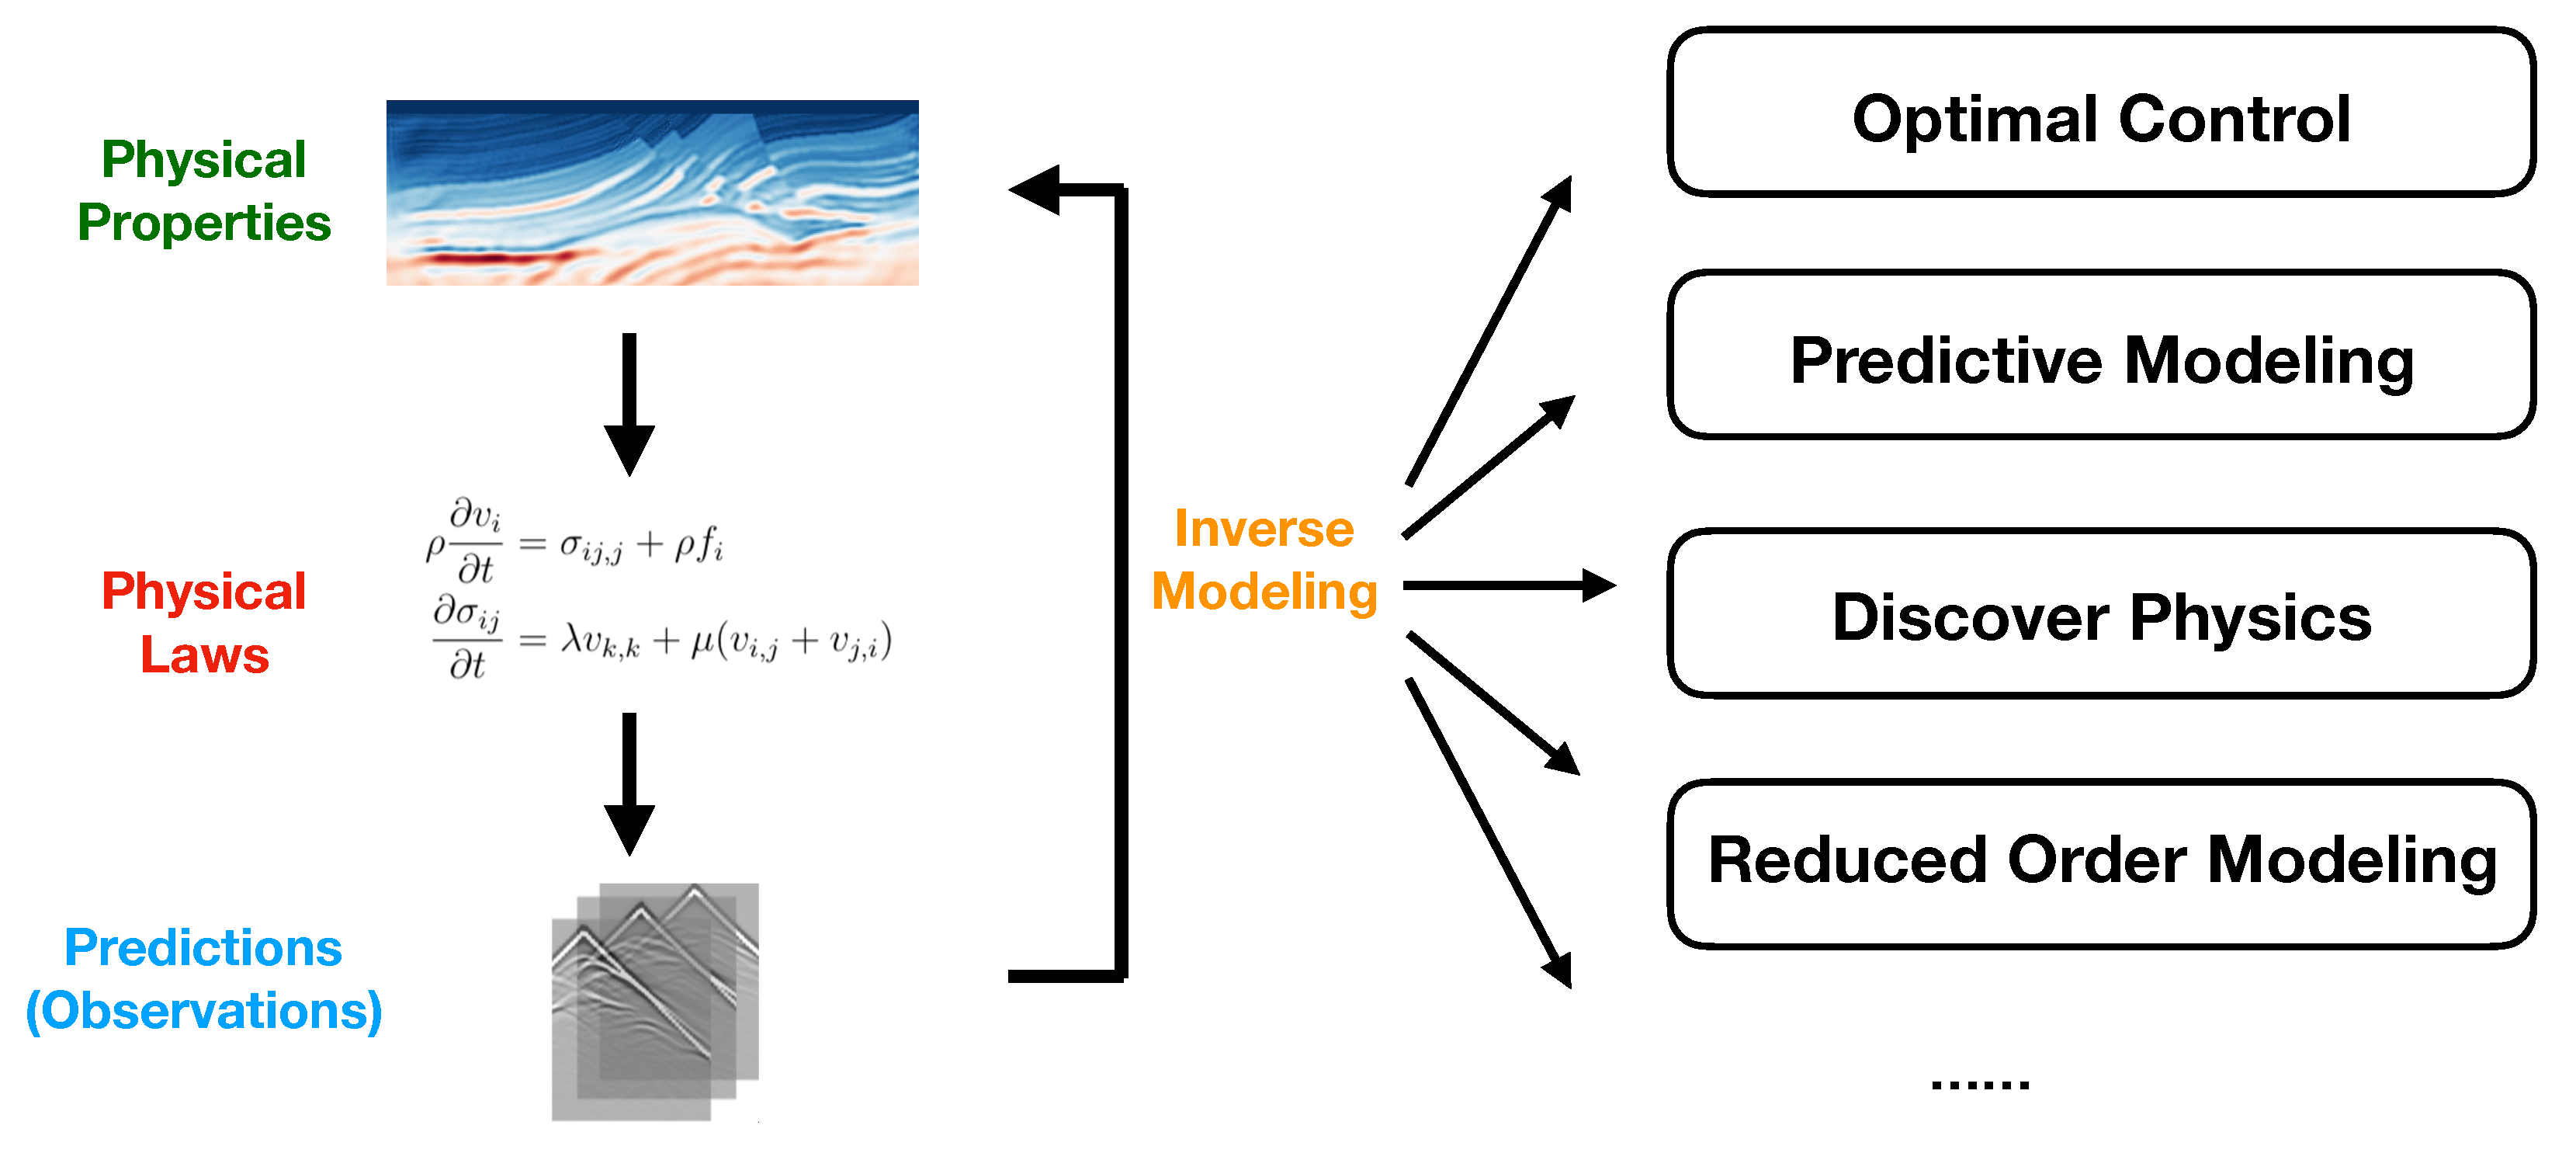
\includegraphics[width=0.8\textwidth]{figures/inverse2}
\end{figure}
\end{frame}


\begin{frame}
	\frametitle{Parameter Inverse Problem}
	\begin{itemize}
		\item The problem we consider so far falls into the category of \textcolor{red}{parameter inverse problem}, where the unknown is one or more parameters. 
		$$\begin{aligned}
\min_{\textcolor{red}{a, b}}\ & \int_{0}^t ( u(0, t)- u_0(t))^2 dt\\
\mathrm{s.t.}\ & \frac{\partial u(x, t)}{\partial t} = \kappa(x)\Delta u(x, t) + f(x, t), \quad t\in (0,T), x\in (0,1) \\
& -\kappa(0)\frac{\partial u(0,t)}{\partial x} = 0, t>0\\
& u(1, t) = 0, t>0\\
& u(x, 0) = 0, x\in [0,1]\\
& \kappa(x) = \textcolor{red}{a} x + \textcolor{red}{b}
\end{aligned}$$

	\end{itemize}
\end{frame}

\begin{frame}
	\frametitle{Function Inverse Problem: Independent of State Variables}
	\begin{itemize}
		\item Another wide category of inverse problem is the so called \textcolor{red}{function inverse problem}, where the unknown is a function. 
		\item First let us consider the case where $\kappa$ is independent of the state variable $u$. 
		$$\begin{aligned}
\min_{\textcolor{red}{\kappa(x)}}\ & \int_{0}^t ( u(0, t)- u_0(t))^2 dt\\
\mathrm{s.t.}\ & \frac{\partial u(x, t)}{\partial t} = \textcolor{red}{\kappa(x)}\Delta u(x, t) + f(x, t), \quad t\in (0,T), x\in (0,1) \\
& -\textcolor{red}{\kappa(0)}\frac{\partial u(0,t)}{\partial x} = 0, t>0\\
& u(1, t) = 0, t>0\\
& u(x, 0) = 0, x\in [0,1]
\end{aligned}$$

	\end{itemize}
\end{frame}

\begin{frame}
	\frametitle{Function Inverse Problem: Dependent on State Variables}
	\begin{itemize}
		\item Another interesting scenario is that $\kappa$ is dependent on $u$. 
		$$\begin{aligned}
\min_{\textcolor{red}{\kappa(x, u)}}\ & \int_{0}^t ( u(0, t)- u_0(t))^2 dt\\
\mathrm{s.t.}\ & \frac{\partial u(x, t)}{\partial t} = \textcolor{red}{\kappa(x, u)}\Delta u(x, t) + f(x, t), \quad t\in (0,T), x\in (0,1) \\
& -\textcolor{red}{\kappa(0, u(0))}\frac{\partial u(0,t)}{\partial x} = 0, t>0\\
& u(1, t) = 0, t>0\\
& u(x, 0) = 0, x\in [0,1]
\end{aligned}$$

	\end{itemize}
\end{frame}

\begin{frame}
	\frametitle{Stochastic Inverse Problem}
	\begin{itemize}
		\item In the fourth category, the unknown is a random variable $\kappa(\varpi)$, where $\varpi$ is the outcome in the probability space. 
		$$\begin{aligned}
\min_{\textcolor{red}{\kappa(\varpi)}}\ & \int_{0}^t ( u(0, t)- u_0(t))^2 dt\\
\mathrm{s.t.}\ & \frac{\partial u(x, t)}{\partial t} = \textcolor{red}{\kappa(\varpi)}\Delta u(x, t) + f(x, t), \quad t\in (0,T), x\in (0,1) \\
& -\textcolor{red}{\kappa(\varpi)}\frac{\partial u(0,t)}{\partial x} = 0, t>0\\
& u(1, t) = 0, t>0\\
& u(x, 0) = 0, x\in [0,1]
\end{aligned}$$

	\end{itemize}
\end{frame}

\begin{frame}
	\frametitle{Four Types of Inverse Problems}
	
	\begin{itemize}
		\item \textcolor{red}{Parameter Inverse Problem}. The unknowns are constant scalars, vectors, matrices, or tensors. $\kappa(x) = a + bx$.
		\item \textcolor{red}{Function Inverse Problem}. The unknowns are functions:
		\begin{itemize}
		\item The unknown function is \textcolor{red}{independent} of state variables. No functional form of $\kappa(x)$ is given. 
		\item The unknown function is \textcolor{red}{dependent} on state variables. No functional form of $\kappa(x, u)$ is given. 
		\end{itemize}
		\item \textcolor{red}{Stochastic Inverse Problem}. The unknown is a random variable. $\kappa(\varpi)$.
	\end{itemize}
	
	This lecture: function inverse problem. 
\end{frame}


% different types of inverse problems
\section{Neural Networks}


\begin{frame}
	\frametitle{Functional Forms}
	
\begin{itemize}
	\item The key to solve function inverse problem is to \textcolor{red}{parametrize} the unknown function $\kappa(x)$ or $\kappa(x, u)$ using a \textcolor{red}{functional form}
	$$\kappa(x) \approx \kappa_\theta(x) \qquad \kappa(x, u) \approx \kappa_\theta(x, u)$$
	\begin{align*}
\min_{\textcolor{red}{\theta}}\ & \int_{0}^t ( u(0, t)- u_0(t))^2 dt\\
\mathrm{s.t.}\ & \frac{\partial u(x, t)}{\partial t} = \textcolor{red}{\kappa_\theta(x)}\Delta u(x, t) + f(x, t), \quad t\in (0,T), x\in (0,1) \\
& -\textcolor{red}{\kappa_\theta(x)}\frac{\partial u(0,t)}{\partial x} = 0, t>0\\
& u(1, t) = 0, t>0\\
& u(x, 0) = 0, x\in [0,1]
\end{align*}

\item Let's see a few functional form examples. 
\end{itemize}
\end{frame}



\begin{frame}

\begin{itemize}
	\item Linear combination of piecewise linear basis functions (``hat functions''). 
	\item The building bricks of finite element analysis (FEA); FEA is the workhorse of many engineering applications (solid mechanics, structural engineering, etc.). 
	$$\kappa_{\theta}(x) = \sum_{i=1}^n c_i\varphi_i(x)\qquad \theta = \{c_i\}_{i=1}^n$$
\end{itemize}

\frametitle{Piecewise Linear Function}
\begin{figure}[hbt]
  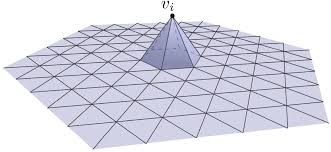
\includegraphics[width=0.45\textwidth]{figures/fe}~
  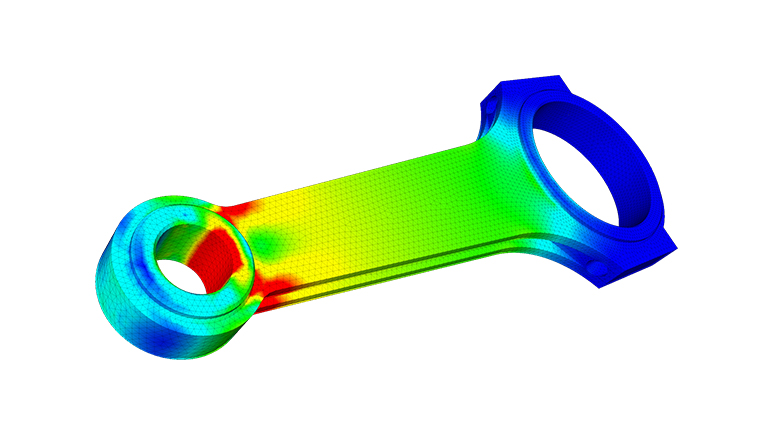
\includegraphics[width=0.45\textwidth]{figures/feapp}
\end{figure}

\end{frame}


\begin{frame}
\frametitle{Radial Basis Function}
\begin{itemize}
	\item A radial basis function depends only on the radial distance from the ``center'' $v_i$ ($\sigma$ is the shape parameter)
	$$\varphi_i(x) = g_{\sigma}(\|x-v_i\|)$$
	\item Linear combination of radial basis functions
	\begin{equation*}
		\kappa_{\theta}(x) = \sum_{i=1}^n c_i\varphi_i(x)\qquad \theta = \{c_i\}_{i=1}^n
	\end{equation*}
\end{itemize}
\begin{figure}[hbt]
  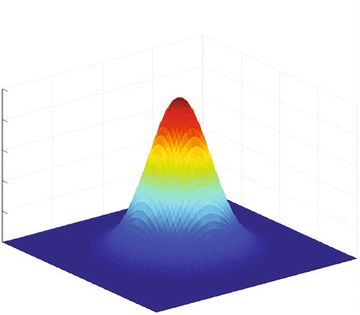
\includegraphics[width=0.3\textwidth]{figures/rbf}~
  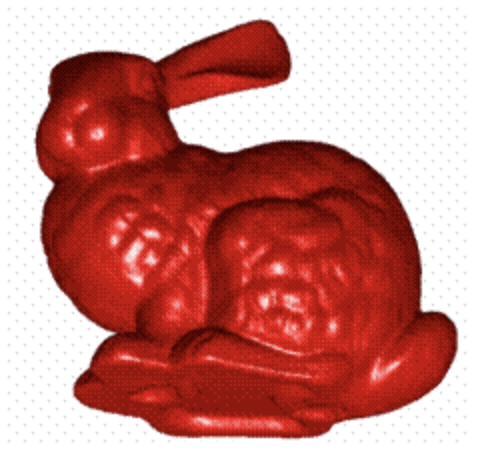
\includegraphics[width=0.3\textwidth]{figures/rbfapp}
\end{figure}

\end{frame}


\begin{frame}
\frametitle{Other Classical Function Approximators}

\begin{itemize}
	\item Most classical function approximators are \red{generalized linear models}. Consider the 1D case
	\begin{equation*}
		\kappa_{\theta}(x) = \sum_{i=1}^n c_i\varphi_i(x)\qquad \theta = \{c_i\}_{i=1}^n
	\end{equation*}
	
	\begin{itemize}
	\item Polynomial regression 
	$$\varphi_i(x) = x^{i-1} $$
	\item Chebyshev polynomials
	$$\varphi_i(x) = \begin{cases}
\cos\big(i \arccos x \big), & \text{if }|x| \le 1 \\
\cosh\big(i \operatorname{arcosh} x \big), & \text{if }x \ge 1 \\ 
(-1)^i \cosh\big(i \operatorname{arcosh} (-x) \big), & \text{if }x \le -1  
\end{cases}$$
\item B-splines
$$\varphi_i(x) = B_{i,p}(x)$$
	\end{itemize}
\end{itemize}
\end{frame}

\begin{frame}
\frametitle{Neural Networks}

\begin{itemize}
	\item Feed-forward neural network
	\begin{equation*}
\left.\begin{aligned}
\by_1 =& \tanh(\mathbf{W}_1 x + \mathbf{b}_1)\\
\by_2 =& \tanh(\mathbf{W}_2 \by_1 + \mathbf{b}_2)\\
\ldots\\
\by_{n-1} =& \tanh(\mathbf{W}_{n-1} \by_{n-2} + \mathbf{b}_{n-1})\\
y =& \mathbf{W}_n \by_{n-1} + \mathbf{b}_n\\
\end{aligned}  \right\} \Rightarrow y = \kappa_{\theta}(x)
\end{equation*}

$$\theta = [\mathbf{W}_1, \mathbf{b}_1, \mathbf{W}_2, \mathbf{b}_2, \ldots, \mathbf{W}_n, \mathbf{b}_n]$$

\item It is another function approximator.
\item It is NOT a linear combination of basis functions: composition of linear functions and nonlinear activation function. 
\end{itemize}

\end{frame}

\begin{frame}
	\frametitle{Neural Networks}

\begin{itemize}
	\item For generalized linear models, the number of coefficients typically grows exponentially in the dimension $d$.
	\item Implementing high dimensional  generalized linear models is nontrivial, but it's often easier to extend neural networks to high dimensional input/output space. 
\end{itemize}
\begin{figure}[hbt]
  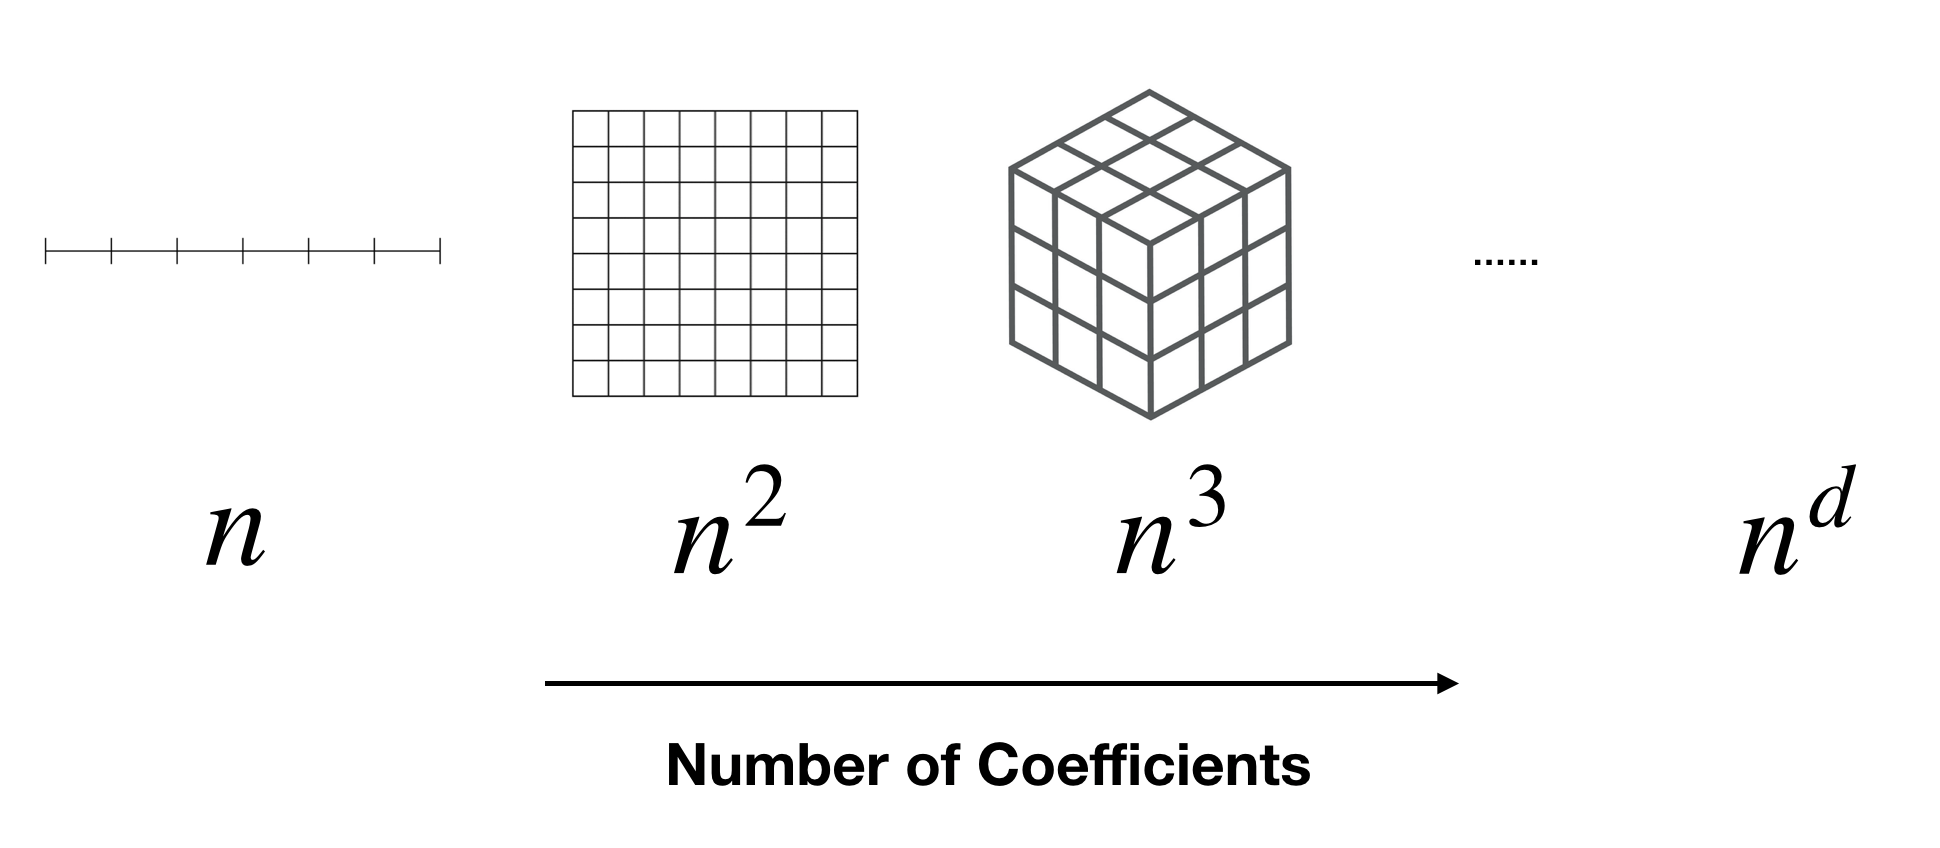
\includegraphics[width=0.8\textwidth]{figures/coef}
\end{figure}


\end{frame}

\begin{frame}


\frametitle{Neural Networks}

\begin{itemize}
	\item Neural network is \red{adaptive} to discontinuities.
\end{itemize}
\begin{figure}[hbt]
  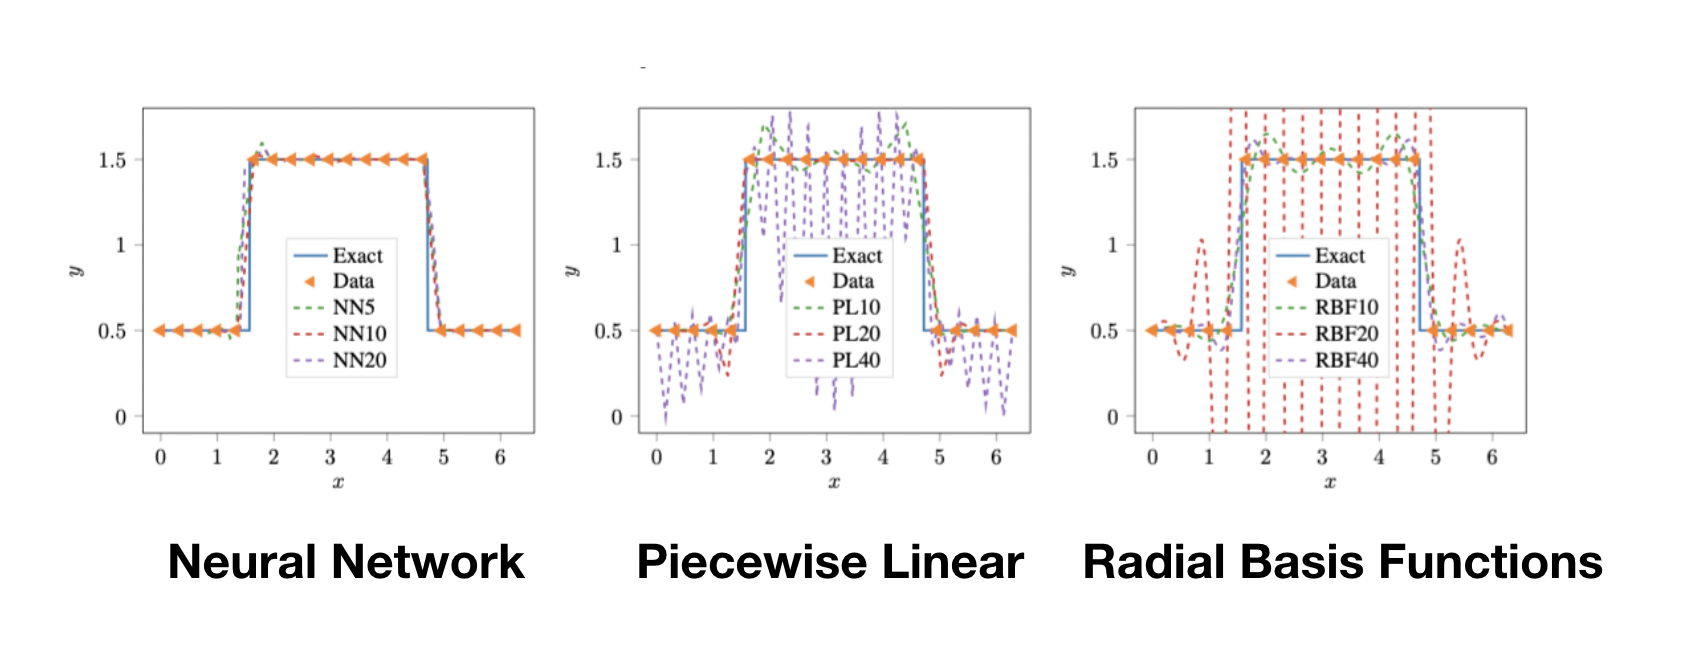
\includegraphics[width=1.0\textwidth]{figures/nn_compare}
\end{figure}

\end{frame}



\begin{frame}

\frametitle{Neural Networks}

\begin{itemize}
	\item Neural network is \red{robust} to noise. Left: NN; right: RBF.
\end{itemize}
\begin{figure}[hbt]
  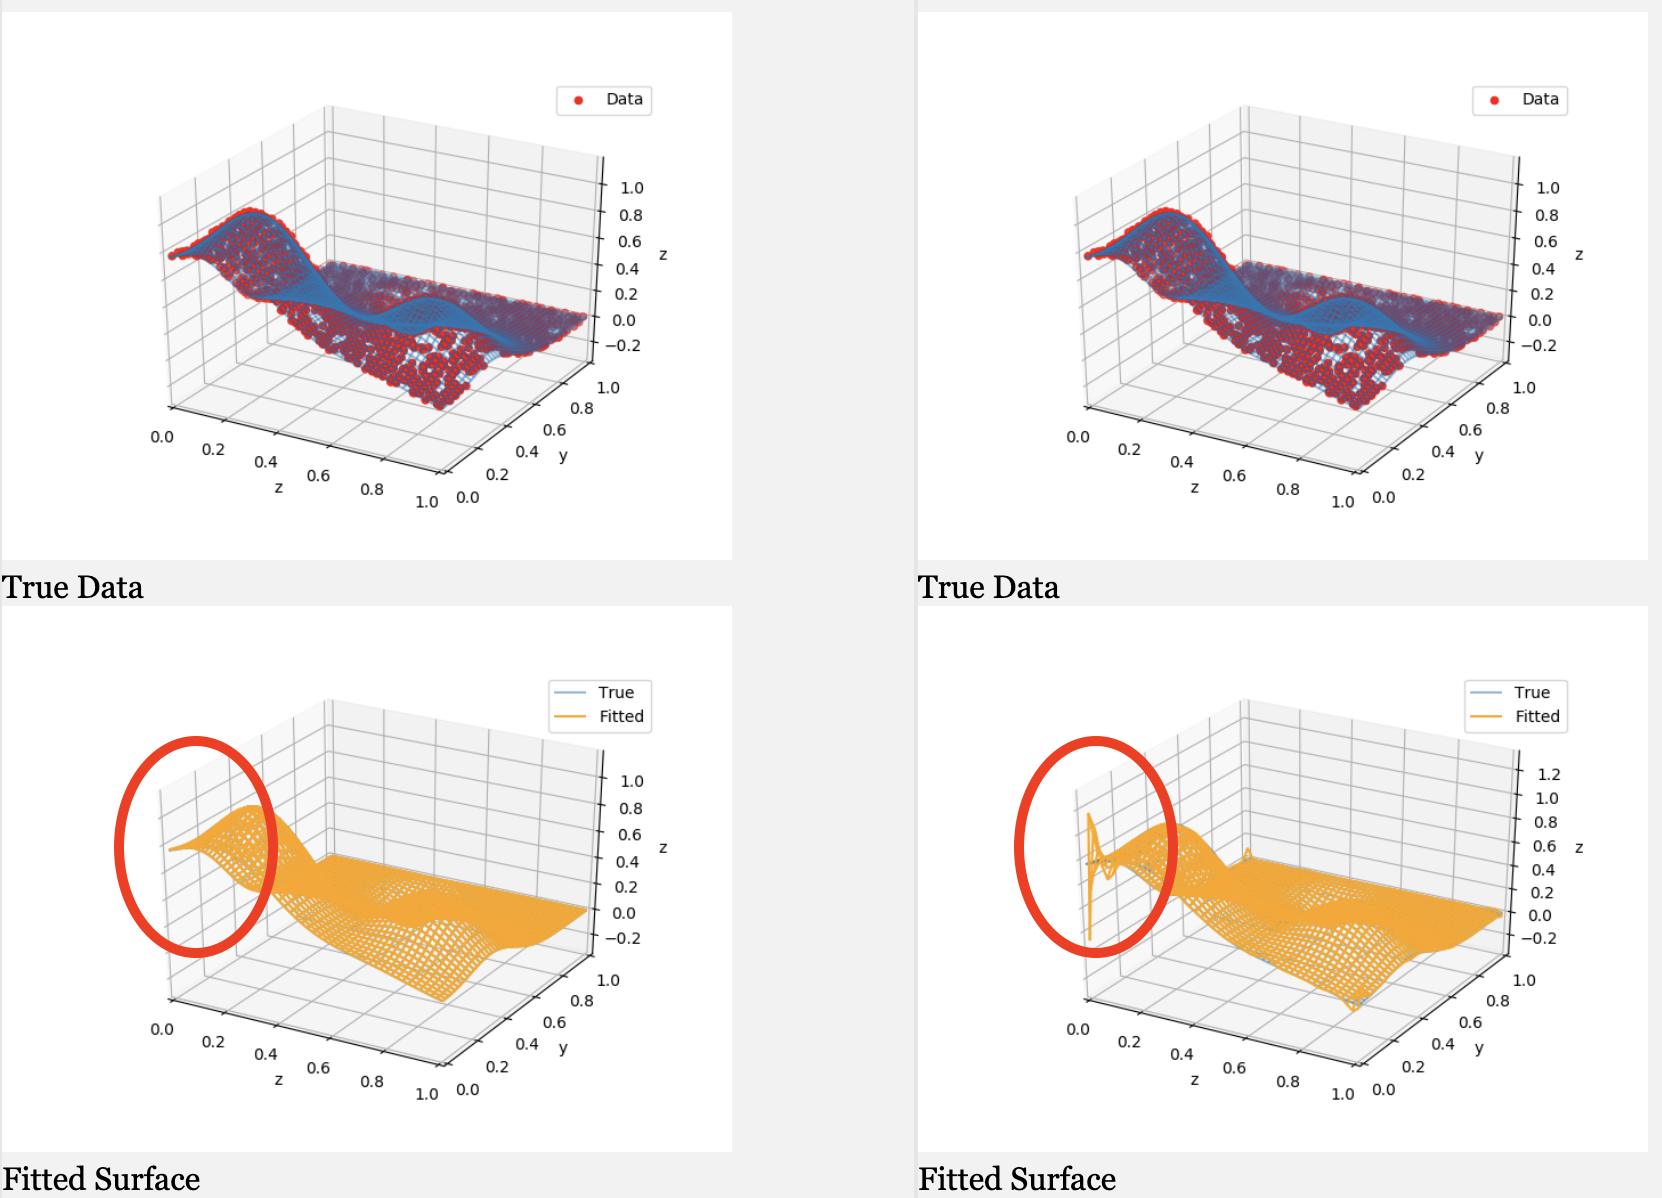
\includegraphics[width=0.8\textwidth]{figures/nn2}
\end{figure}

\end{frame}


\begin{frame}

\frametitle{Neural Networks}

\begin{itemize}
	\item \red{Quasi-Newton optimization} (when it is affordable) is more efficient than stochastic gradient descent methods. Left: BFGS; right: SGD. 
	\begin{figure}[hbt]
  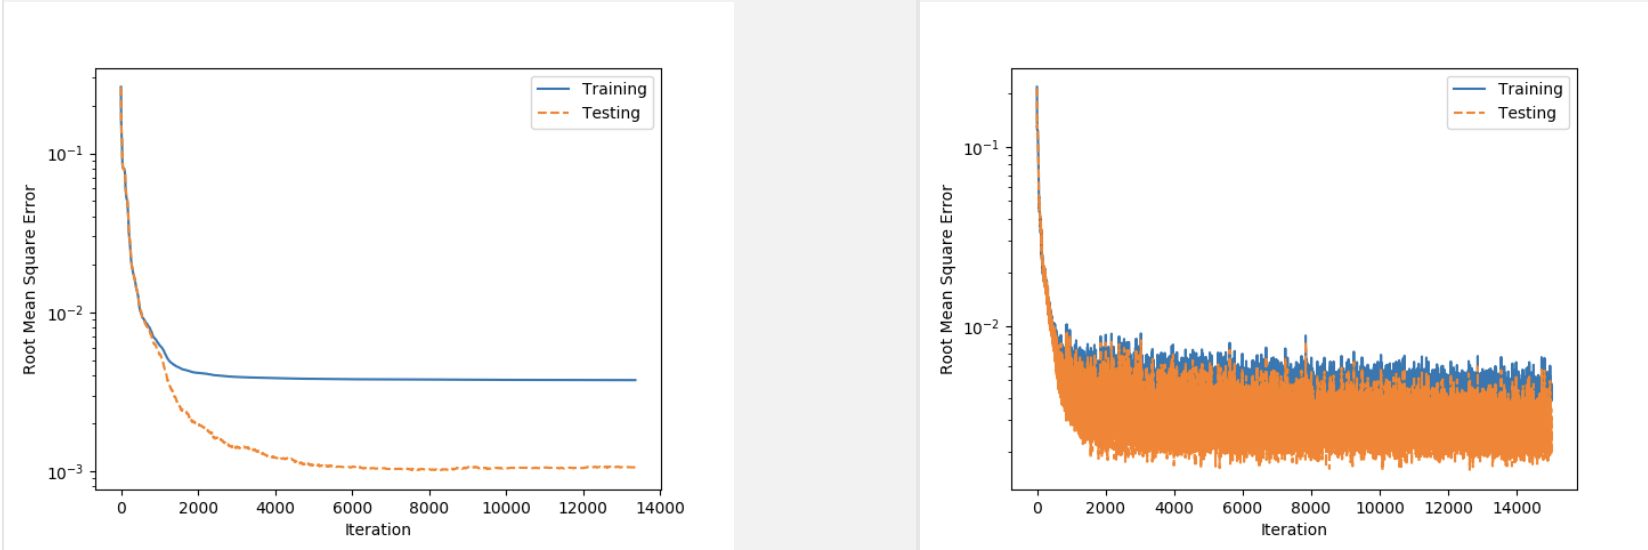
\includegraphics[width=0.8\textwidth]{figures/opt}
\end{figure}

\end{itemize}

\end{frame}

\begin{frame}
	\frametitle{Take-Home Messages}
	
	\begin{itemize}
	\item Neural network is easily extended to \textcolor{red}{high dimensions}. 
		\item Neural network exhibits \red{adaptiveness} for discontinuous functions, compared to function approximators with fixed basis functions.
		\item Neural network is more \red{robust} to noise than traditional global basis functions such as radial basis functions. 
		\item \red{(Quasi-)second-order} optimizers converge faster and are more stable than stochastic gradient descent methods, as long as you can afford the computational and memory cost.
	\end{itemize}
\end{frame}




\begin{frame}
	\frametitle{Use Neural Networks to Parametrize Unknown Functions}
	
\begin{itemize}
	\item Substitute $\kappa(x)$ with a neural network $\kappa_\theta(x)$, and then solve the PDE-constrained optimization problem:
	\begin{align*}
\min_{\textcolor{red}{\theta}}\ & \int_{0}^t ( u(0, t)- u_0(t))^2 dt\\
\mathrm{s.t.}\ & \frac{\partial u(x, t)}{\partial t} = \textcolor{red}{\kappa_\theta(x)}\Delta u(x, t) + f(x, t), \quad t\in (0,T), x\in (0,1) \\
& -\textcolor{red}{\kappa_\theta(0)}\frac{\partial u(0,t)}{\partial x} = 0, t>0\\
& u(1, t) = 0, t>0\\
& u(x, 0) = 0, x\in [0,1]
\end{align*}
\item Major technical difficulty: how to train the neural networks (estimate $\theta$)?
\end{itemize}
\end{frame}




\begin{frame}
	\frametitle{Computational Graph}
	
	\begin{itemize}
		\item The computational graphs of a neural network and a  numerical solver are coupled. 
		\begin{figure}[hbt]
  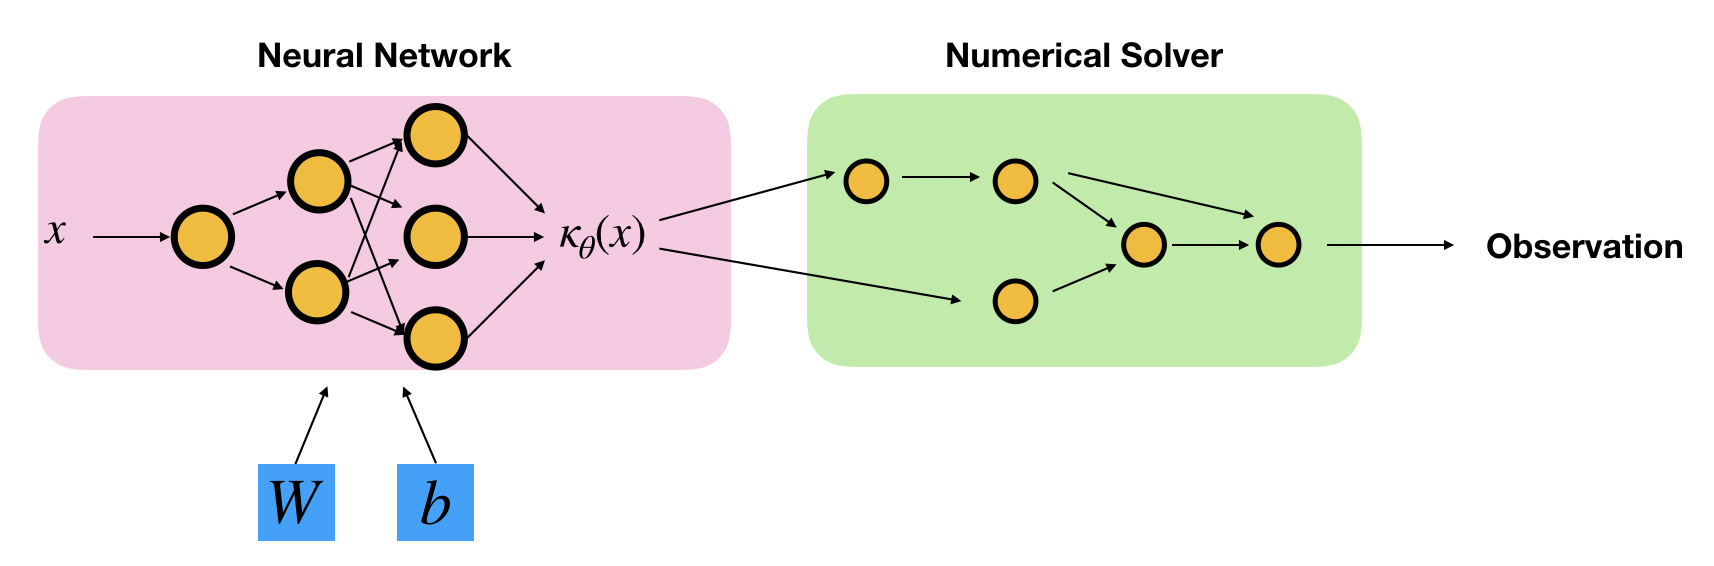
\includegraphics[width=0.8\textwidth]{figures/solver}
\end{figure}
		\item  Training Neural Networks: estimating the weights and biases of the neural network $W, b$ by running gradient descent on the computational graph. 
	\end{itemize}

\end{frame}



\begin{frame}
	\frametitle{Computational Graph for Numerical Schemes}
	
	\begin{itemize}
		\item The discretized optimization problem is 
		\begin{align*}
			\min_{\theta}& \; \sum_{k=1}^m (u^k_1 - u_0( (k-1)\Delta t))^2\\
			\text{s.t.} & \; A(\theta)U^{k+1} = U^k + F^{k+1}, k = 1, 2,\ldots, m \\
			& \; U^0 = 0
		\end{align*}
		\item The computational graph for the forward computation (evaluating the loss function) is 
		\begin{figure}[hbt]
		\centering
  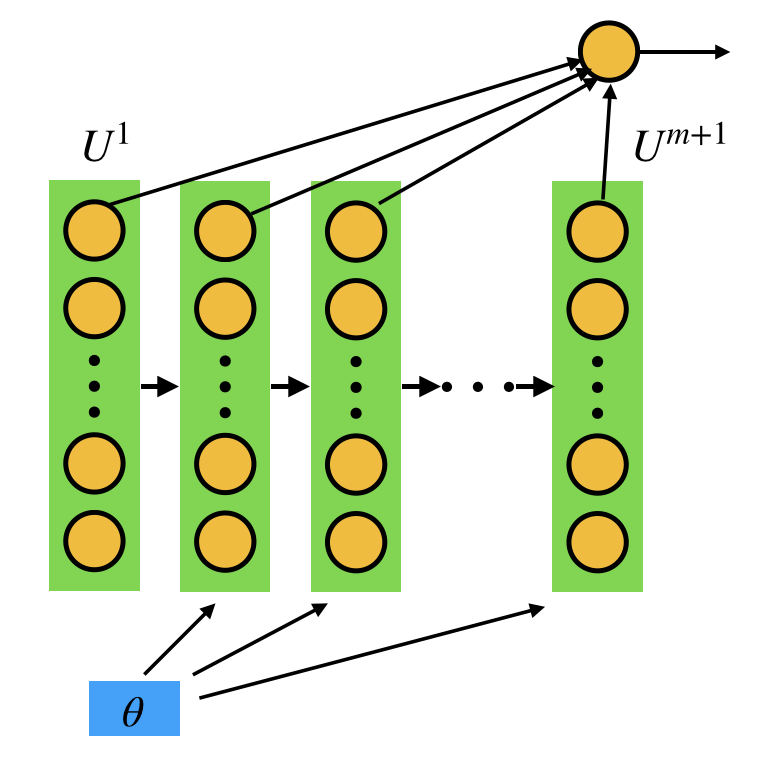
\includegraphics[width=0.3\textwidth]{figures/heatcg2}
\end{figure}

	\end{itemize}
\end{frame}


% an illustrative example

\section{Training Algorithms}

\begin{frame}
	\frametitle{Direct Training}
	
	\begin{itemize}
		\item If the input and output pairs
		$$\{(u_i, x_i), \kappa_i\}_{i=1}^n$$
		to $\kappa_\theta(u,x)$ are available, we can train the neural network using the standard supervised learning method
	$$\min_\theta\ \sum_{i=1}^n (\kappa_\theta(u_i, x_i) - \kappa_i)^2$$
	\item Pros:
	\begin{itemize}
	\item Extremely easy to implement using a deep learning software. 
	\item No insight from the PDE is required.
	\end{itemize}
	\item Cons:
	\begin{itemize}
	\item Input-output pair data may not be available.
	\item Leads to nonphysical $\kappa_\theta$ by ignoring the PDE. 
	\end{itemize}
	\end{itemize}
\end{frame}

\begin{frame}
	\frametitle{Residual Minimization}
	\begin{itemize}
		\item Assumption: the full field data of the state variable $u(x, t)$ are available. Possible in laboratories. 
		\begin{figure}[hbt]
		\centering
  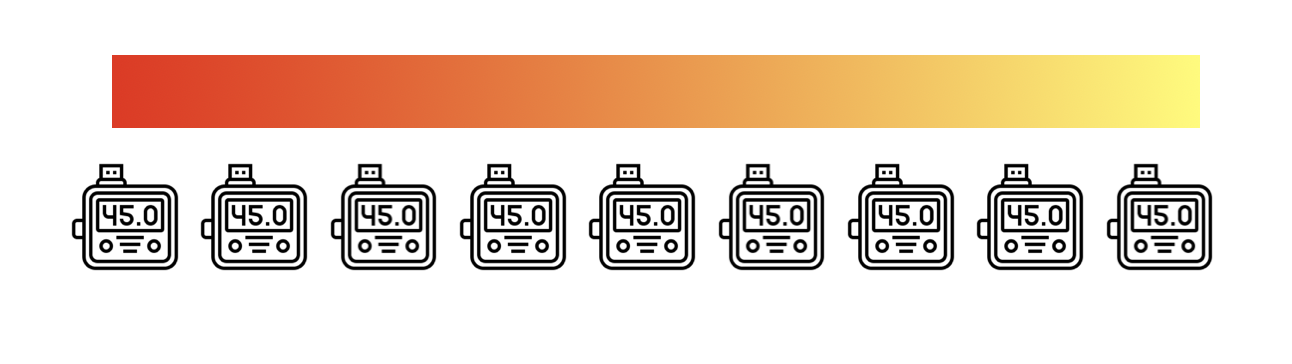
\includegraphics[width=0.8\textwidth]{figures/fullfield}
\end{figure}

\item Solve an unconstrained optimization problem:

$$\min_\theta \ \sum_{j}\sum_{i=1}^n \left(\frac{\partial u}{\partial t}\Big|_{x = x_i, t = t_j} - \left( {\kappa_\theta(x)}\Delta u + f\right)\Big|_{x = x_i, t = t_j}\right)^2$$
	\end{itemize}
\end{frame}

\begin{frame}
	\frametitle{Residual Minimization}
	\begin{itemize}
		\item Pros:
		\begin{itemize}
		\item No insight is required into numerical solvers; however, insight into the PDE is required. 
		\item Do not require input-output pair data. 
		\end{itemize}
		\item Cons:
		\begin{itemize}
		\item Full field data is required. 
		\item Does not enforce the PDE constraints (the residual may not be zero due to local minimum).
		\end{itemize}
		
	\end{itemize}
\end{frame}

\begin{frame}
	\frametitle{Penalty Method}
	
	\begin{itemize}
		\item Solve the constrained optimization problem using the penalty method
		\begin{align*}
\min_{\textcolor{red}{u},\theta} &  \int_{0}^t ( u(0, t)- u_0(t))^2 dt \\
& + \textcolor{red}{\lambda_1} \int_{0}^t \int_{0}^1 \left(\frac{\partial u(x, t)}{\partial t} - {\kappa_\theta(x, u)}\Delta u(x, t) - f(x, t)\right)^2 dtdx\\
&	+  \textcolor{red}{\lambda_2}\int_0^t \int_0^1	\left(-{\kappa_\theta(x, u)}\frac{\partial u(0,t)}{\partial x}\right)^2 dtdx \\
& +  \textcolor{red}{\lambda_3}\int_0^t u(1, t)^2 dt+   \textcolor{red}{\lambda_4}\int_0^1 u(x, 0)^2 dx
		\end{align*}
	Here $\lambda_1$, $\lambda_2$, $\lambda_3$ and $\lambda_4$ are positive penalty parameters. 

	\end{itemize}
\end{frame}


\begin{frame}
	\frametitle{Penalty Method}
	\begin{itemize}
		\item Pros:
		\begin{itemize}
		\item No insight is required into numerical solvers; however, insight into the PDE is required. 
		\item Do not require input-output pair data. 
		\item Do not require knowing $u$ everywhere (a.k.a., sparse observations)
		\end{itemize}
		\item Cons:
		\begin{itemize}
		\item The number of free optimization variables increase by the degrees of freedom (DOF) of state variable. This may be an issue for dynamic problems, where the DOF is very large (solution vectors at each time step must be added to free optimization variables). 
		\item Does not enforce the PDE constraints.
		\item Selecting appropriate $\lambda_i$'s is challenging. 
		\item Convergence is an issue for stiff problems. 
		\end{itemize}
		
	\end{itemize}
\end{frame}


\begin{frame}
	\frametitle{Physics Constrained Learning (Optional)}
	\begin{center}
\textcolor{red}{\mbox{An efficient and powerful approach for} \\\mbox{ automatic differentiation through implicit numerical schemes}}
	\end{center}
	\begin{itemize}
		\item Physics constrained learning (PCL) solves for $u$ first in the PDE constrained optimization. 
	\end{itemize}
	\begin{itemize}
\item[Step1] Solve for $u$
\begin{align*}
 \frac{\partial u(x, t)}{\partial t} &= {\kappa_\theta(x)}\Delta u(x, t) + f(x, t), \quad t\in (0,T), x\in (0,1) \\
-{\kappa_\theta(x)}\frac{\partial u(0,t)}{\partial x} &= 0, t>0\\
 u(1, t) &= 0, t>0\\
 u(x, 0) &= 0, x\in [0,1]
\end{align*}
	\end{itemize}
	$$\boxed{u = u_\theta(x, t)}$$
\end{frame}


\begin{frame}
	\frametitle{Physics Constrained Learning (Optional)}
	
	\begin{itemize}
\item[Step2] Solve the unconstrained optimization problem
\begin{align*}
 \min_\theta \ \tilde L_h(\theta) := \int_{0}^t ( u_\theta(0, t)- u_0(t))^2 dt
\end{align*} 
This step requires computing the gradients
$$\boxed{\frac{\partial \tilde L_h(\theta)}{\partial \theta}}$$
\end{itemize}

However, wse cannot express $u_\theta$ analytically in terms of $\theta$.

\textbf{Challenge}: how to compute the gradient \textcolor{red}{efficiently} and \textcolor{red}{automatically} in a computational graph?

\end{frame}



\begin{frame}
	\frametitle{Physics Constrained Learning (Optional)}
\begin{itemize}
	\item Let's consider a simple example
	\begin{align*}
		\min_\theta & \ \|u-u_0\|^2\\
		\mathrm{s.t.} & \ (A+\theta B) u = y 
	\end{align*}
	
	By definition:
	$$\tilde L_h(\theta) := \|u_\theta-u_0\|^2$$
	where $u_\theta$ is the solution to 
	$$ (A+\theta B) u = y $$
\end{itemize}	

\end{frame}


\begin{frame}
	\frametitle{Recap: Implicit Function Theorem}
	
	\begin{itemize}
		\item Consider a function $f:x\mapsto y$, implicitly defined by 
		$$x^3-(y^3+y) = 0$$
		\item Treat $y$ as a function of $x$ and take the derivative on both sides
		$$3x^2 - 3y(x)^2y'(x)-y'(x)=0$$
\item Rearrange the expression and we obtain 
$$y'(x) = \frac{3x^2}{3y(x)^2+1}$$
	\end{itemize}
	
\end{frame}


\begin{frame}
	\frametitle{Physics Constrained Learning}
	\begin{enumerate}
		\item 
		$$\frac{\partial \tilde L_h(\theta)}{\partial \theta} = 2(u_\theta-u_0)^T \frac{\partial u_\theta}{\partial \theta}$$
\item To compute $\frac{\partial u_\theta}{\partial \theta}$, consider the PDE constraint ($\theta$ is a scalar)
$$B(\theta) u_\theta = y$$
Take the derivative with respect to $\theta$ on both sides 
$$\frac{\partial B(\theta)}{\partial \theta}u_\theta + B(\theta) \frac{\partial u_\theta}{\partial \theta} = 0\Rightarrow \frac{\partial u_\theta}{\partial \theta} = -B(\theta)^{-1} \frac{\partial B(\theta)}{\partial \theta}u_\theta$$
\item Finally, 
$$\frac{\partial \tilde L_h(\theta)}{\partial \theta} = -2(u_\theta-u_0)^TB(\theta)^{-1} \frac{\partial B(\theta)}{\partial \theta}u_\theta$$
	\end{enumerate}
\end{frame}

\begin{frame}
	\frametitle{Physics Constrained Learning}
	
	\begin{enumerate}
		\item Remember: in reverse-mode AD, gradients are always back-propagated from downstream (objective function) to upstream (unknowns). 
		\item The following quantity is computed first:
		$$g^T = 2(u_\theta-u_0)^TB(\theta)^{-1}$$
		which is equivalent to solve a linear system 
		$$B(\theta)^T g = 2(u_\theta-u_0)$$
		\item \textcolor{red}{In the gradient back-propagation step, a linear system with an adjoint matrix (compared to the forward computation) is solved.} 
		\item Finally, 
		$$\frac{\partial \tilde L_h(\theta)}{\partial \theta} = -2(u_\theta-u_0)^TB(\theta)^{-1} \frac{\partial B(\theta)}{\partial \theta}u_\theta = -g^T \frac{\partial B(\theta)}{\partial \theta}u_\theta$$
	\end{enumerate}
\end{frame}


\begin{frame}
	\frametitle{Physics Constrained Learning}
	
	\begin{itemize}
		\item A trick for evaluating $g^T Bu_\theta$: consider $g$ as independent of $\theta$ in the computational graph, then 
		$$g^T \frac{\partial B(\theta)}{\partial \theta}u_\theta = \frac{\partial (g^T B(\theta) u_\theta)}{\partial \theta}$$
		\item $g^T B(\theta) u_\theta$ is a scalar, thus we can apply reverse-mode AD to compute $g^T B(\theta) u_\theta$.
		\item Declaring independence of variables can be done with \texttt{tf.stop\_gradient} in TensorFlow or \texttt{independent} in ADCME. 
	\end{itemize}
\end{frame}




\begin{frame}
	\frametitle{Physics Constrained Learning (Optional)}
	 $${\small    \min_{\theta}\; L_h(u_h) \quad \mathrm{s.t.}\;\; F_h(\theta, u_h) = 0}$$
	\begin{itemize}
\item Assume in the forward computation, we solve for $u_h=G_h(\theta)$ in $F_h(\theta, u_h)=0$, and then
$${\small\tilde L_h(\theta)  = L_h(G_h(\theta))}$$
\item Applying the \textcolor{red}{implicit function theorem}
{  \scriptsize
\begin{equation*}
\frac{{\partial {F_h(\theta, u_h)}}}{{\partial \theta }} + {\frac{{\partial {F_h(\theta, u_h)}}}{{\partial {u_h}}}}  \frac{\partial G_h(\theta)}{\partial \theta} = 0  \Rightarrow 
     \frac{\partial G_h(\theta)}{\partial \theta} =  -\Big( \frac{{\partial {F_h(\theta, u_h)}}}{{\partial {u_h}}} \Big)^{ - 1} \frac{{\partial {F_h(\theta, u_h)}}}{{\partial \theta }}
\end{equation*}
}
\item Finally we have
{\scriptsize
\begin{equation*}
    \boxed{\frac{{\partial {{\tilde L}_h}(\theta )}}{{\partial \theta }} 
    = \frac{\partial {{ L}_h}(u_h )}{\partial u_h}\frac{\partial G_h(\theta)}{\partial \theta}= - \frac{{\partial {L_h}({u_h})}}{{\partial {u_h}}} \;
    \Big( {\frac{{\partial {F_h(\theta, u_h)}}}{{\partial {u_h}}}\Big|_{u_h = {G_h}(\theta )}} \Big)^{ - 1} \;
    \frac{{\partial {F_h(\theta, u_h)}}}{{\partial \theta }}\Big|_{u_h = {G_h}(\theta )}}
\end{equation*}
}

	\end{itemize}
	
\end{frame}

\begin{frame}
	\frametitle{Summary}
	We compare the residual minimization method, penalty method, and physics constrained learning (PCL) from several aspects. We exclude the direct training method due to its limitation to input-output pairs. 

\begin{figure}[hbt]
\centering
  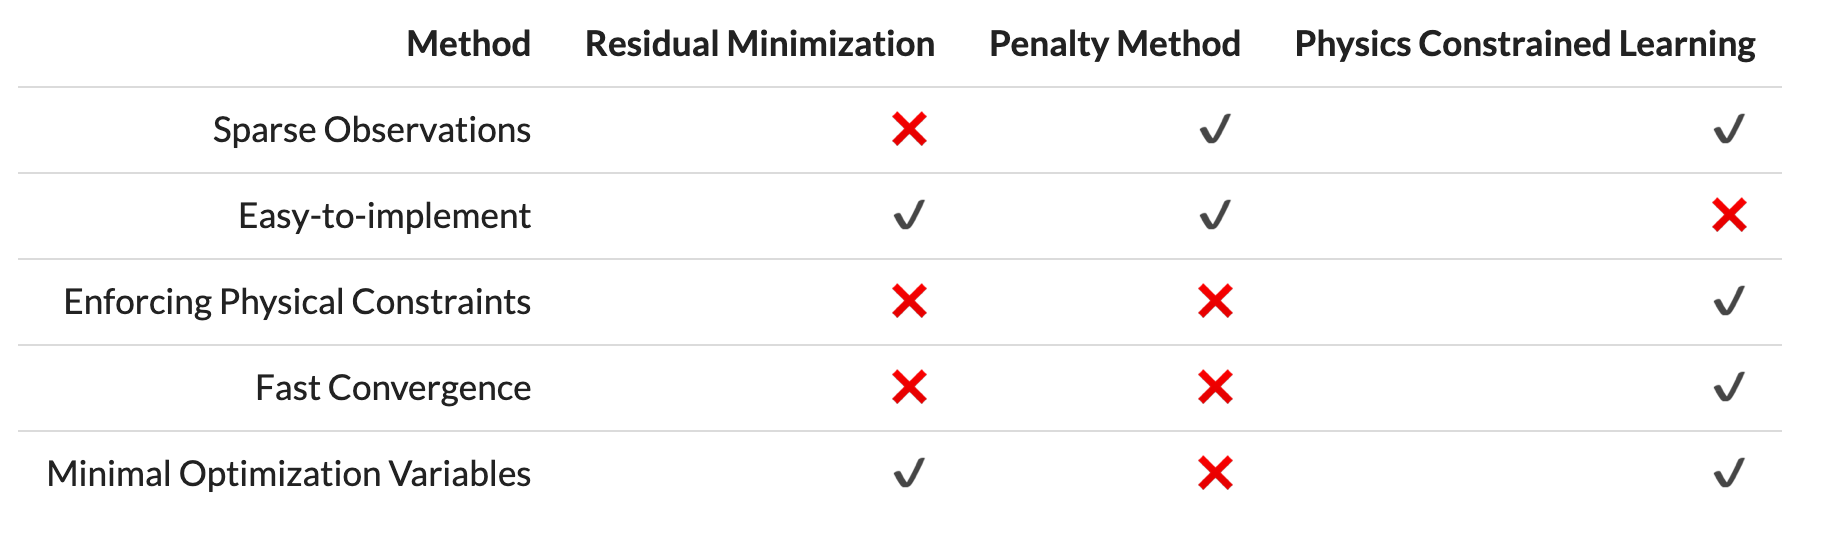
\includegraphics[width=1.0\textwidth]{figures/comparetrain}
\end{figure}

\end{frame}


\section{ADCME}

\begin{frame}
	\frametitle{An Overview}
	
	\begin{itemize}
		\item The ADCME library (Automatic Differentiation Library for Computational and Mathematical Engineering) aims at general and scalable \textcolor{red}{inverse modeling} in \textcolor{red}{scientific computing} with \textcolor{red}{gradient-based optimization} techniques.
		\item The automatic differentiation engine: \textcolor{red}{TensorFlow static graph mode}. 
		\begin{figure}[hbt]
  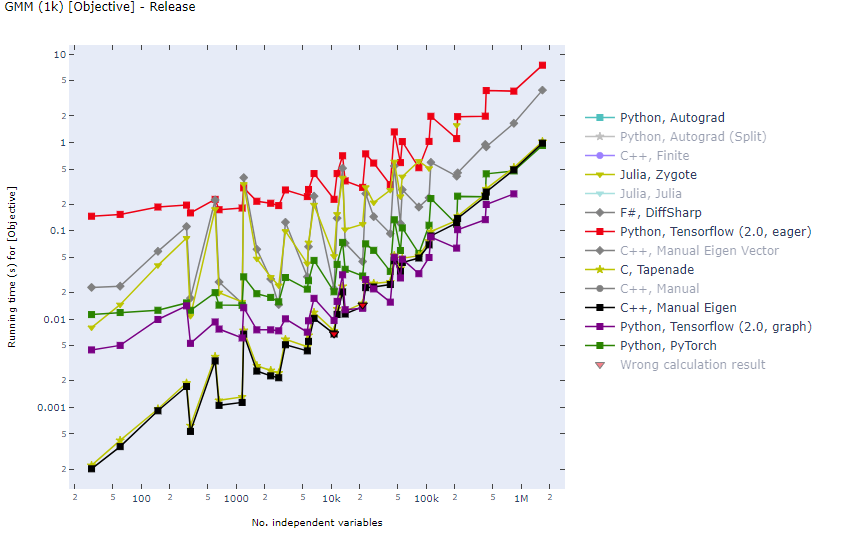
\includegraphics[width=0.8\textwidth]{figures/reverseAD}
\end{figure}

	\end{itemize}
\end{frame}


\begin{frame}
	\frametitle{How ADCME works?}
	
	\begin{itemize}
		\item Uses TensorFlow for computational graph-based optimization and generation of the computational graph for calculating gradients.
		\item Provides optimized C++ kernels and interfaces that are essential for scientific computing. Featured modules:
		\begin{itemize}
		\item Sparse Linear Algebra Library. 
		\item Custom Optimizer, such as Ipopt and NLopt. 
		\item Neural Network with Tangent Matrices (sensitivity). See \texttt{fc} for details. 
		\item Probabilistic Metrics for stochastic inverse problems, such as \texttt{dtw} and \texttt{sinkhorn}.
		\end{itemize}
		
		  
	\end{itemize}
	
	\begin{figure}[hbt]
	\centering
  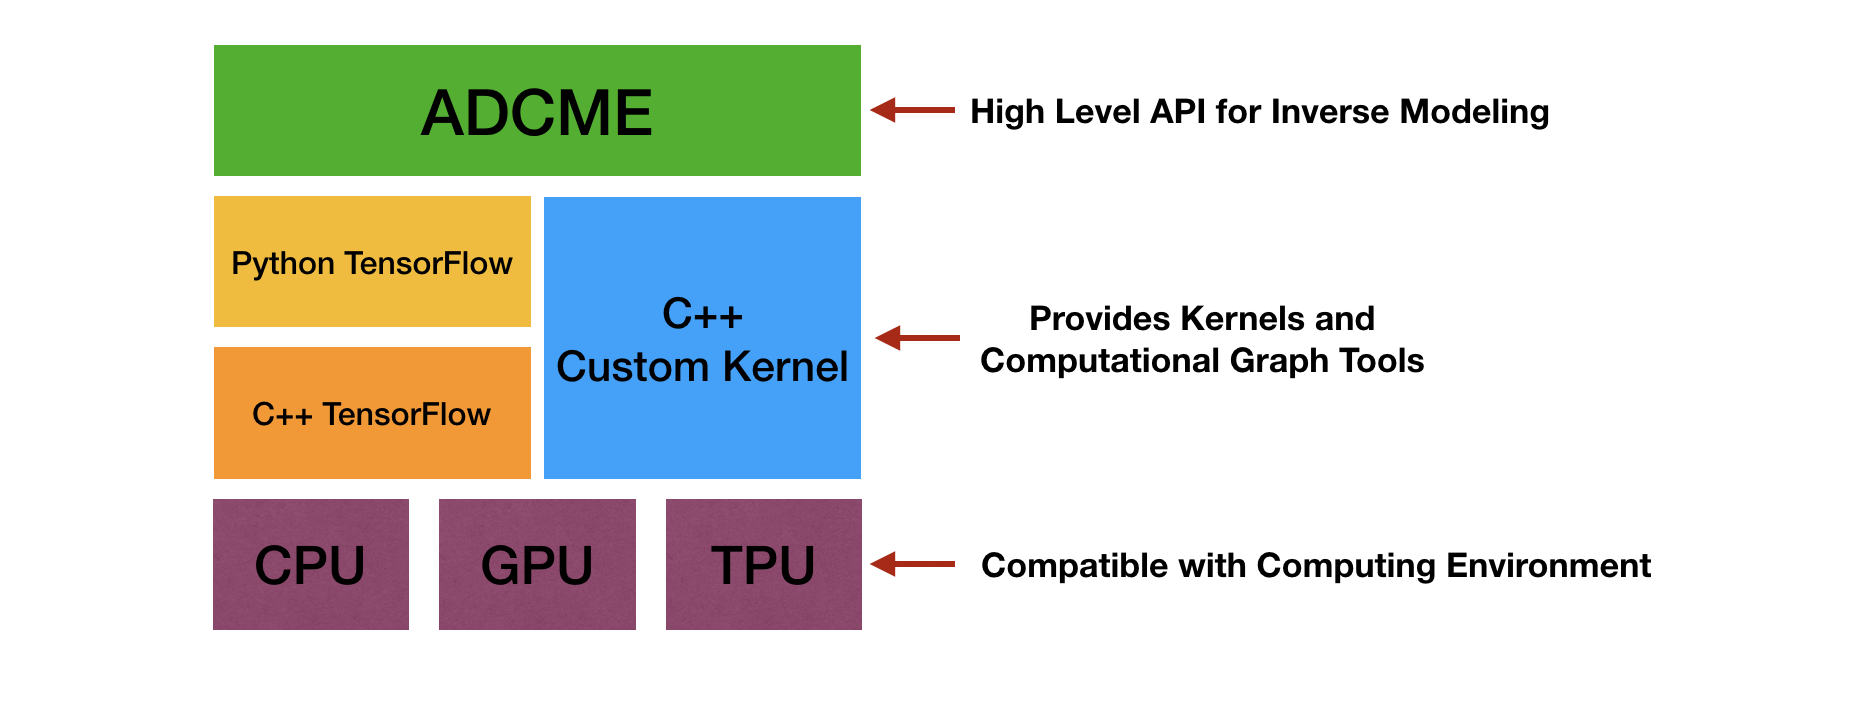
\includegraphics[width=0.8\textwidth]{figures/kernel2}
\end{figure}

\end{frame}
\begin{frame}
	\frametitle{Featured Applications (Optional)}
	
	Before we have some hands-on experience with inverse modeling using ADCME, let's first see some applications. 
\end{frame}

\begin{frame}
	\frametitle{ADSeismic.jl: A General Approach to Seismic Inversion}
	\begin{itemize}
		\item Solve seismic inversion problems within a unified framework. 
	\end{itemize}
	\begin{figure}[hbt]
  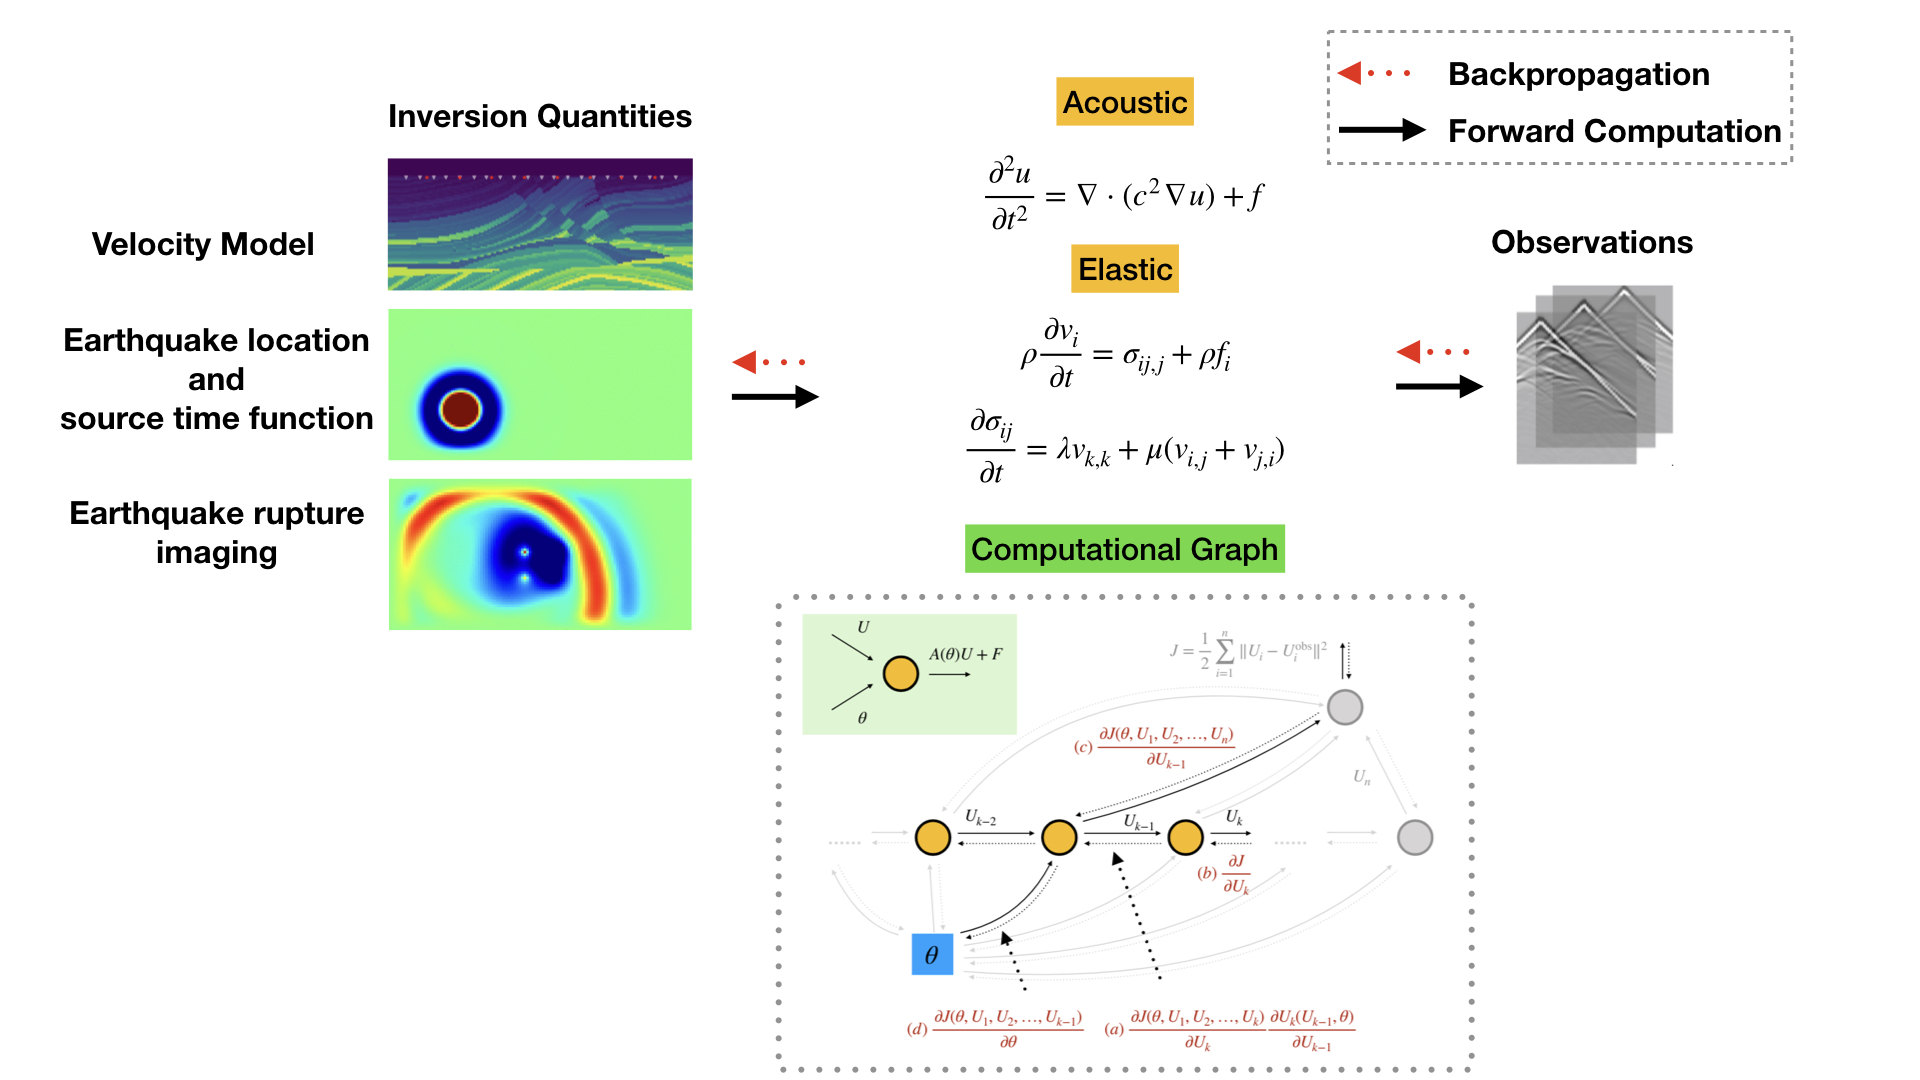
\includegraphics[width=1.0\textwidth]{figures/adseimic.jpeg}
\end{figure}
	
\end{frame}

\begin{frame}
	\frametitle{FwiFlow.jl: Coupled Full Waveform Inversion for Subsurface Flow Problems}
	\begin{itemize}
		\item Estimating hydrological properties from high resolution geological data (e.g., seismic data). 
	\end{itemize}
	\begin{figure}[hbt]
  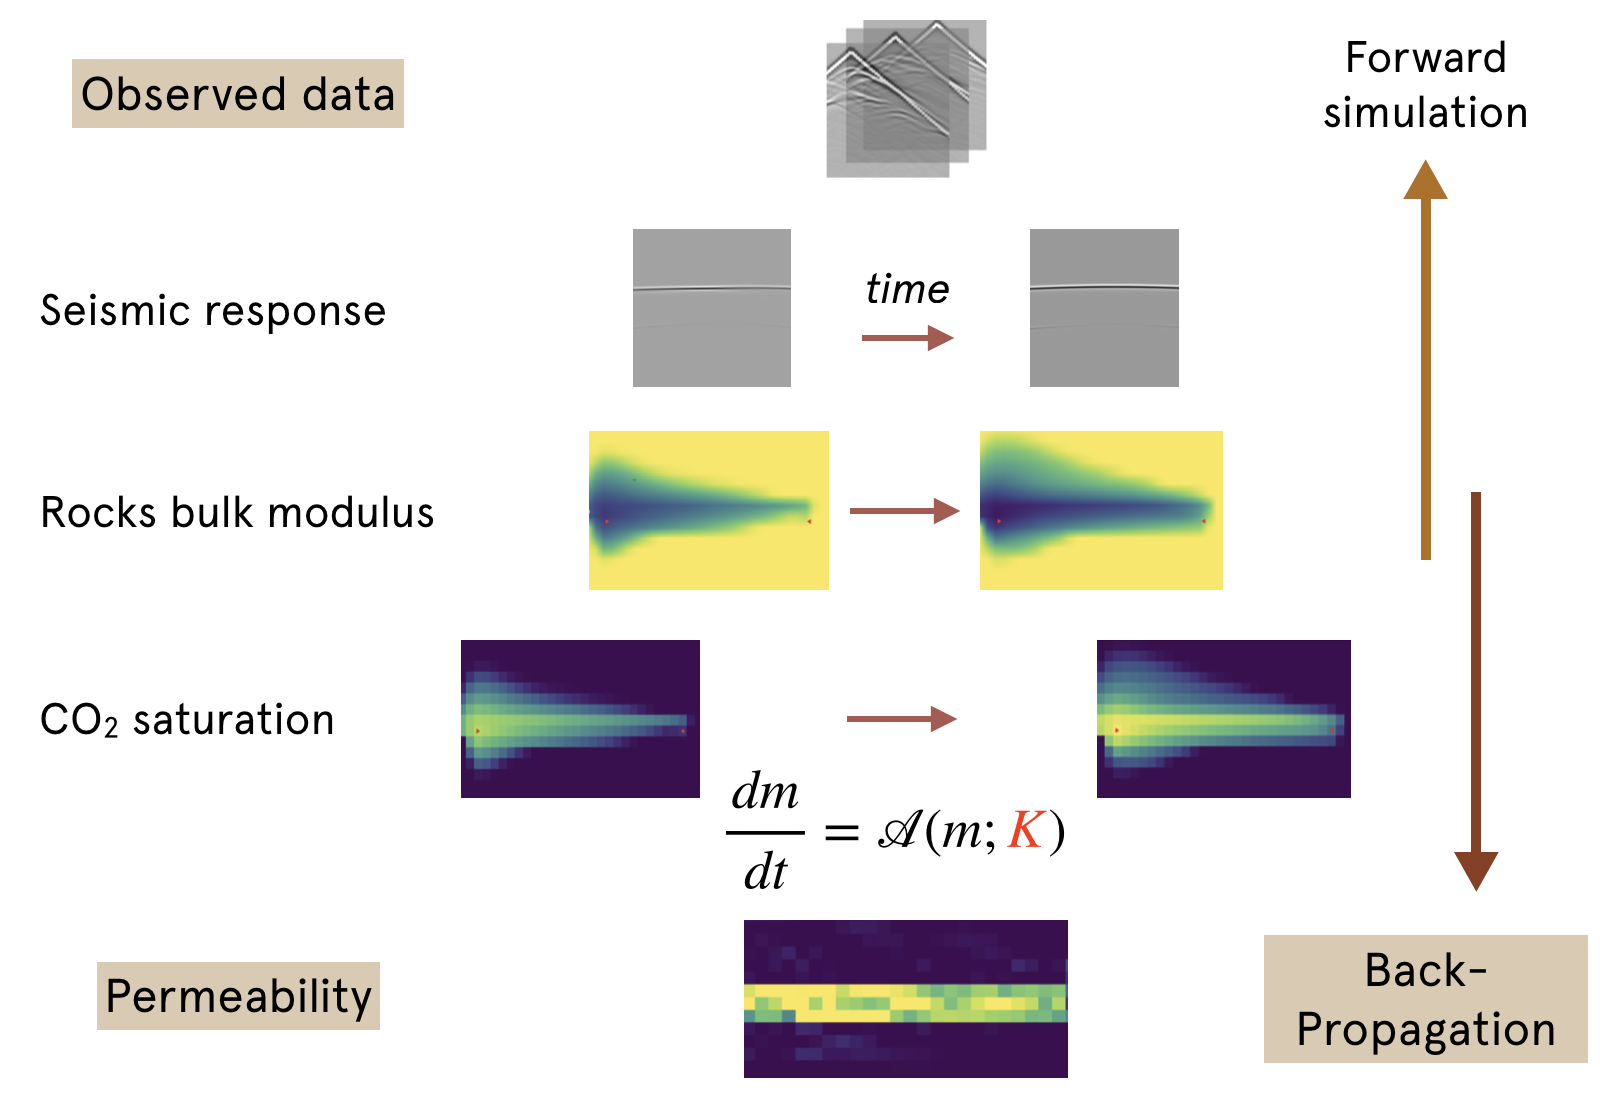
\includegraphics[width=0.6\textwidth]{figures/geo.png}
\end{figure}
\end{frame}

\begin{frame}
	\frametitle{NNFEM.jl: Robust Constitutive Modeling}
	\begin{itemize}
	\item Modeling constitutive relations in dynamic structural equations using neural networks. 
	\item A finite element library built on computational graph. 

	\end{itemize}

\begin{center}
	\begin{minipage}[t]{0.48\textwidth}
\begin{figure}[hbt]
\centering
  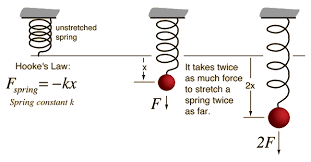
\includegraphics[width=1.0\textwidth]{figures/hook}
\end{figure}
\end{minipage}
\begin{minipage}[t]{0.48\textwidth}	
\begin{figure}[hbt]
\centering
  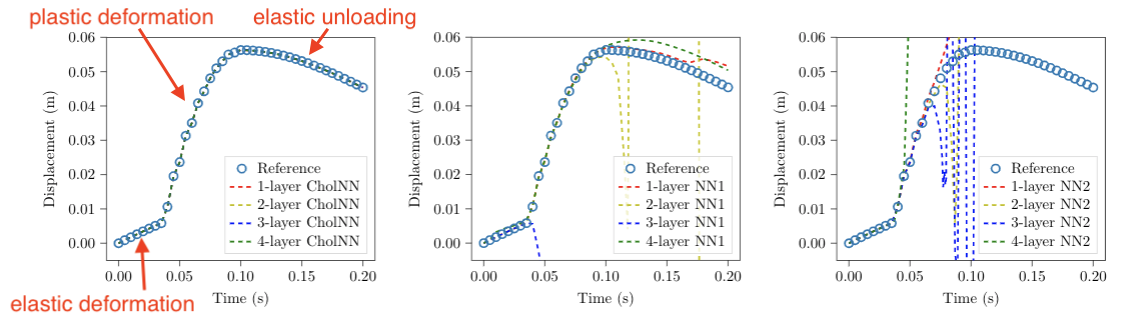
\includegraphics[width=1.0\textwidth]{figures/nncons}
\end{figure}
\end{minipage}
\end{center}


{\scriptsize Image source: \url{http://hyperphysics.phy-astr.gsu.edu/hbase/permot2.html}}
\end{frame}

\begin{frame}
	\frametitle{ADCME Example}
	\begin{center}
		Hands-on Example
	\end{center}
\end{frame}

\section{Conclusion}


\begin{frame}
	\frametitle{Conclusion}
	\begin{itemize}
		\item What's covered in this lecture
		\begin{itemize}
		\item Four types of inverse problems: 
		\begin{itemize}
			\item Parameter inverse problem;
			\item function inverse problem (covered in this lecture);
			\item Stochastic inverse problem.
		\end{itemize}
		\item Neural networks as a function approximation form;
		\item Training algorithms:
		\begin{itemize}
		\item Direct training;
		\item Residual minimization;
		\item Penalty method;
		\item Physics constrained learning.
		\end{itemize}
		\item ADCME: applications and hands-on examples
		\end{itemize}
	\end{itemize}
\end{frame}



\end{document} 